\documentclass[11pt]{article}
\usepackage[T1]{fontenc}
\usepackage{lmodern}
\usepackage[utf8]{inputenc}
\usepackage{amsmath,amssymb,amsthm}
\usepackage{graphicx,booktabs,array,longtable}
\usepackage[margin=1in]{geometry}
\usepackage{microtype}
\usepackage[hidelinks]{hyperref}
\usepackage{xcolor}
\newtheorem{theorem}{Theorem}
\newtheorem{proposition}{Proposition}
\newtheorem{lemma}{Lemma}
\newtheorem{corollary}{Corollary}
\theoremstyle{definition}
\newtheorem{definition}{Definition}
\newtheorem{prediction}{Prediction}
\theoremstyle{remark}
\newtheorem{remark}{Remark}
\newcommand{\grade}[1]{\textsc{[#1]}}
\renewcommand{\arraystretch}{1.15}
\title{The Twin-Prime Chain in the Peel Ball\\[4pt]\large Endpoint Law, Frame Turn, the Thread Cut by Every Prime,\\ and Where the Turn Is Set}
\author{Jeromie Beasley}
\date{24 November 2026 \quad (version 2)}
\begin{document}
\maketitle

\begin{center}\small\emph{Prepared with AI assistance (Claude). Every number in this paper comes from a script listed in Appendix~B.}\end{center}

\begin{abstract}
The twin-prime starts $11,17,29,41,\dots$ are walked through the peel ball as a product of Lorentz boosts. Each step has rapidity $r=\ln(a'/a)$, so its peel reflection is $\Gamma=(z-1)/(z+1)=\tanh(r/2)$ with $z=a'/a$. The step runs along one of three perpendicular arms, chosen by the end digit $1,7,9$ of the next twin start, which is exactly its class $11,17,29 \pmod{30}$. Six results are established.
\begin{enumerate}
\item \emph{The exact step.} The step and its turn have an exact form at any arm angle $\gamma$: $\tan(\varepsilon/2)=\Gamma_1\Gamma_2\sin\gamma/(1+\Gamma_1\Gamma_2\cos\gamma)$. The wall where two equal steps stop composing into a rotation sits at $\Gamma^2=1/(1+\sin\gamma)$, which is $\Gamma^2=\tfrac12$ for perpendicular arms.
\item \emph{The endpoint law.} The distance grows as $d=|P|\,L+c$, where $L=\ln(a/11)$ is the path and $P$ is the gap-weighted mean arm. This is proved under two weak conditions. For the three cube arms $|P|=1/\sqrt3$, and $c=0.1086$ is measured to $10^{12}$.
\item \emph{The frame turn is a holonomy.} Each step's turn is the area it sweeps in rapidity space. A convergence theorem for the frame is proved under named conditions. A proof without those conditions would itself settle an open twin-prime statement.
\item \emph{The tilt is derived.} The small end-digit tilt that steers the heading off the cube diagonal is derived from the Hardy--Littlewood local factors (the thread of the twin chain cut by every prime). It matches the twin primes in every decade from $10^5$ to $10^{12}$.
\item \emph{The turn limit.} The frame turn is $12.3442^\circ$ at $10^{12}$, and the readout of the turn once the tilt dies is $12.46508^\circ$, stable from $10^{10}$ on.
\item \emph{Connection energy.} The forward and reversed readings of the same chain disagree by a connection energy $\|[L,L^*]\|/\|L\|^2$ that levels off near $0.13$.
\item \emph{Where the turn is set.} A curvature dial and its opposite setup show that the turn is set by the walk's first steps, not at the wall crossing. The wall reading is killed in both setups.
\item \emph{Other prime pairs.} Cousin and sexy primes, with one arm rule (the residue mod~$5$), share the slope $1/\sqrt3$ and the early wall crossing. The turn is not a Hardy--Littlewood quantity: twins and cousins share the constant but differ by $2.7^\circ$.
\item \emph{The dodecahedral honeycomb.} The twin arms are the edges of the $\{5,3,4\}$ honeycomb, whose edge has $\cosh\ell=\varphi$ and $\Gamma^2=\sqrt5-2$. Two perpendicular edges turn the frame by exactly $\arctan\tfrac12$. Walked on the honeycomb, the order of the twin end digits alone shows a prime signal at $z=-51$; about $16\%$ of it is memory beyond consecutive pairs.
\item \emph{Two predictions of version 1 settled.} The $7/9$ split offset and the cousin tilt both pass.
\item \emph{The 186 bound.} The main terms of OpenAI's certificate are confirmed independently. The gap $182$ is out of reach with their inputs.
\end{enumerate}
A closing section reads these results against a view of light as the fixed stage and the electron as the mover. That section is interpretation, and is labelled as such.
\end{abstract}

\tableofcontents
\bigskip

\noindent\textbf{Grades.} Every statement carries one grade:
\begin{itemize}
\item \grade{proved}: exact algebra, also checked numerically;
\item \grade{derived}: follows from stated inputs, with an approximation named;
\item \grade{conditional}: proved under a named hypothesis;
\item \grade{measured}: computed on the twin primes;
\item \grade{cited}: a published result;
\item \grade{untested}: a prediction with its kill condition written down.
\end{itemize}

%=====================================================
\section{Introduction}

The peel step of VOTKP reads a ratio $z$ as a reflection,
\[
\Gamma=\frac{z-1}{z+1}=\tanh\!\left(\tfrac12\ln z\right).
\]
In \emph{Two Trees in One Ball}, two perpendicular steps of equal size compose into a boost and a turn. The turn is the Thomas turn, $\tan(\theta/2)=\Gamma^2$. The pair stops composing into a pure rotation at the wall $\Gamma^2=\tfrac12$, that is $z=3+2\sqrt2$, where $\operatorname{tr}[A,B]=2-4\sinh^4(r/2)$ reaches $-2$.

This paper puts the twin primes into that ball. Each twin start is a step. Its size is the log of the ratio to the previous start, and its direction is set by its end digit. The questions are:
\begin{itemize}
\item where the chain goes;
\item how much its frame turns;
\item what steers it;
\item what the two readings of one chain, forward and reversed, have to say to each other.
\end{itemize}

The answers join several pieces of the framework:
\begin{itemize}
\item the peel step and the wall (VOTKP);
\item the turn as curvature (the intrinsic, non-Riemannian geometry of the ball);
\item connection energy as non-normality;
\item the shrinking ruler of \emph{Matter at a Scale};
\item the electron and light as the two parts of one dance.
\end{itemize}

%=====================================================
\section{The chain}

\begin{definition}[Twin chain]
Let $a_0=11<a_1<a_2<\cdots$ be the twin-prime starts above $5$ (so $a$ and $a+2$ are both prime). For $n\ge1$:
\begin{itemize}
\item the step size is $r_n=\ln(a_n/a_{n-1})$, with ratio $z_n=a_n/a_{n-1}$ and peel reflection $\Gamma_n=\tanh(r_n/2)=(z_n-1)/(z_n+1)$;
\item the arm $e_{s_n}\in\{e_x,e_y,e_z\}$ is chosen by the end digit of $a_n$: $1\mapsto e_x$, $7\mapsto e_y$, $9\mapsto e_z$.
\end{itemize}
\end{definition}

\begin{proposition}[Arms are classes mod 30] \grade{proved}
Every twin start $a>5$ satisfies $a\equiv 11,17,29\pmod{30}$, and the end digits $1,7,9$ match these three classes one to one.
\end{proposition}
\begin{proof}
For $a$ and $a+2$ to both be prime above $5$:
\begin{itemize}
\item $a$ is odd;
\item $a\not\equiv 1\pmod 3$, since otherwise $3\mid a+2$; so $a\equiv 2\pmod3$;
\item $a\not\equiv 0,3\pmod 5$.
\end{itemize}
By the Chinese remainder theorem the classes mod 30 are $11,17,29$. Their end digits are $1,7,9$.
\end{proof}

Let $B(e,r)$ be the Lorentz boost of rapidity $r$ along $e$. The chain is the product
\[
L_n=B(e_{s_1},r_1)\,B(e_{s_2},r_2)\cdots B(e_{s_n},r_n),
\]
with polar split $L_n=\mathrm{Boost}(d_n\,n_n)\,R_n$. Its parts are:
\begin{itemize}
\item the distance $d_n$;
\item the heading $n_n$, the lab view;
\item the frame $R_n$;
\item the body heading $u_n=R_n^{\mathsf T}n_n$.
\end{itemize}
The path is $L=\sum r_k=\ln(a_n/11)$.

In spinors, $B(e,r)$ is $H=\cosh(r/2)+\sinh(r/2)\,e\cdot\sigma$, and the chain lives in $SL(2,\mathbb C)$. The position in the Poincar\'e ball is $\tanh(d/2)\,n$. Figure~\ref{fig:ball} shows the chain to $10^6$.

%=====================================================
\section{The exact step and the wall}

\begin{proposition}[Polar factor] \grade{proved}
If $M=HU$ with $H$ a boost, $U$ a rotation and $\det M=1$, then
\[
U=\frac{M+M^{\dagger\,-1}}{\operatorname{tr}H}.
\]
\end{proposition}
\begin{proof}
\begin{itemize}
\item $M^{\dagger-1}=H^{-1}U$, because $H^\dagger=H$ and $U^{\dagger-1}=U$.
\item By Cayley--Hamilton for $\det H=1$: $H+H^{-1}=(\operatorname{tr}H)\,I$.
\item Hence $M+M^{\dagger-1}=(H+H^{-1})U=(\operatorname{tr}H)\,U$.
\end{itemize}
\end{proof}

\begin{proposition}[Composition of two boosts] \grade{proved}
Take two boosts with rapidities $\zeta_1,\zeta_2$ along directions at angle $\gamma$, and write $\Gamma_i=\tanh(\zeta_i/2)$. Their product is a boost times a rotation by $\varepsilon$ about the axis normal to both directions, with
\[
\tan\frac{\varepsilon}{2}=\frac{\Gamma_1\Gamma_2\sin\gamma}{1+\Gamma_1\Gamma_2\cos\gamma}
=\frac{\sin\gamma}{\coth(\zeta_1/2)\coth(\zeta_2/2)+\cos\gamma}.
\]
The resulting rapidity satisfies
\[
\cosh d'=\cosh\zeta_1\cosh\zeta_2+\sinh\zeta_1\sinh\zeta_2\cos\gamma .
\]
\end{proposition}
\begin{proof}
Write $c_i=\cosh(\zeta_i/2)$ and $s_i=\sinh(\zeta_i/2)$, and take unit directions $n$ and $w$. Then
\[
M+M^{\dagger-1}=2\bigl[c_1c_2+s_1s_2\cos\gamma+i\,s_1s_2\,(n\times w)\cdot\sigma\bigr].
\]
A rotation by $\varepsilon$ is $\cos(\varepsilon/2)-i\sin(\varepsilon/2)\,a\cdot\sigma$. Reading off its two parts and dividing by $c_1c_2$ gives the first formula. The second is the time component of the composed boost.
\end{proof}

\noindent\emph{Checks.} At 160 digits the worst errors are:
\begin{itemize}
\item $10^{-146}$ for the turn;
\item $6\times10^{-160}$ for the distance;
\item $2\times10^{-111}$ for the body-frame update.
\end{itemize}
An independent double-precision check over 100 random pairs agrees to $7\times10^{-14}$. For perpendicular equal steps the formula reduces to $\tan(\varepsilon/2)=\Gamma^2$, the Thomas turn of \emph{Two Trees in One Ball}.

\begin{corollary}[Step expansion] \grade{proved}
For a walker at distance $d$ taking a step $r$ at angle $\theta$ to its heading,
\[
\varepsilon=r\tanh\frac d2\,\sin\theta-\frac{r^2}{2}\tanh^2\frac d2\,\sin\theta\cos\theta+O(r^3).
\]
\end{corollary}
\noindent The remainder divided by $r^3$ is $-0.03267$ at both $r=10^{-4}$ and $r=10^{-6}$.

\begin{proposition}[The wall at any angle] \grade{proved}
For $A=\exp(\tfrac{r_1}{2}e\cdot\sigma)$ and $B=\exp(\tfrac{r_2}{2}m\cdot\sigma)$ with $e\cdot m=\cos\gamma$,
\[
\operatorname{tr}[A,B]=2-4\sinh^2\frac{r_1}{2}\sinh^2\frac{r_2}{2}\sin^2\gamma .
\]
For equal steps the wall $\operatorname{tr}[A,B]=-2$ sits at
\[
\Gamma^2=\frac{1}{1+\sin\gamma}.
\]
\end{proposition}
\begin{proof}
\begin{enumerate}
\item Fricke's identity: $\operatorname{tr}[A,B]=\operatorname{tr}^2A+\operatorname{tr}^2B+\operatorname{tr}^2AB-\operatorname{tr}A\operatorname{tr}B\operatorname{tr}AB-2$.
\item Substitute $\operatorname{tr}A=2c_1$, $\operatorname{tr}B=2c_2$ and $\operatorname{tr}AB=2(c_1c_2+s_1s_2\cos\gamma)$.
\item Expand. The cross terms in $\cos\gamma$ cancel, leaving $4c_1^2+4c_2^2-4c_1^2c_2^2+4s_1^2s_2^2\cos^2\gamma-2$.
\item With $c^2=1+s^2$ this is $2-4s_1^2s_2^2\sin^2\gamma$.
\item At the wall, $s^4\sin^2\gamma=1$, so $s^2=1/\sin\gamma$ and $\Gamma^2=s^2/(1+s^2)=1/(1+\sin\gamma)$.
\end{enumerate}
Numerical check: the worst error over 100 random cases is $1.4\times10^{-14}$.
\end{proof}

\noindent\emph{The twin chain and the wall} \grade{measured}:
\begin{itemize}
\item No single step reaches the wall below $10^9$. The largest is $17\to29$, with $\Gamma^2=0.068$ (Figure~\ref{fig:wall}).
\item The chain as a whole crosses the wall sphere $\rho^2=\tfrac12$ (with $\rho=\tanh(d/2)$) between the twin starts $197$ and $227$. By then $80\%$ of its final turn already exists.
\item Read as three books (each arm's steps summed into one boost), the pairs of arms reach the wall at the twin starts $1151$ $(x,z)$, $2027$ $(y,z)$ and $4481$ $(x,y)$.
\end{itemize}

%=====================================================
\section{The frame-free form}

\begin{proposition}[Distance and heading run on their own] \grade{proved}
Every boost is symmetric, so $L_n^{\mathsf T}=B_nL_{n-1}^{\mathsf T}$. The vector
\[
Y_n=L_n^{\mathsf T}e_0=(\cosh d_n,\ \sinh d_n\,u_n)
\]
obeys $Y_n=B(e_{s_n},r_n)\,Y_{n-1}$, with $Y_0=e_0$.
\end{proposition}

\noindent So distance and body heading form a walk of their own, and the frame is driven by them. Like a two-shaft gearbox, the inner shaft (distance and heading) turns by itself, and the outer sleeve (the frame) rides on it.

\begin{proposition}[Octant] \grade{proved}
In velocity form $v=\tanh(d)\,u$, a step along arm $s$ is relativistic velocity addition:
\[
v_s'=\frac{v_s+\tanh r}{1+v_s\tanh r},\qquad v_\perp'=\frac{v_\perp}{\cosh r\,(1+v_s\tanh r)}.
\]
Both maps keep every component non-negative. Since $v_0=0$, $v$ stays in the closed positive octant of the unit ball.
\end{proposition}

%=====================================================
\section{The endpoint law}

\begin{theorem}[Endpoint law] \grade{conditional}
Assume the following.
\begin{itemize}
\item[(A1)] $r_n\to0$.
\item[(A2)] For every fixed window of path length $T$, the window sums of $r_k(e_{s_k}-p_\infty)$ tend to $0$, for some limit weights $p_\infty$.
\end{itemize}
Write $P_\infty=\sum_s p_{\infty,s}\,e_s$. Then $u_n\to P_\infty/|P_\infty|$, $d_n\to\infty$, and $d_n/L\to|P_\infty|$. The condition $\sum r_n^2<\infty$ is not needed.
\end{theorem}

\begin{proof}[Outline]
\begin{enumerate}
\item In velocity form, $v_{n+1}=v_n+r_n[F(v_n)+U_n]+O(r_n^2)$, with $F(v)=P-(P\cdot v)v$ and noise $U_n=(I-vv^{\mathsf T})(e_{s_n}-P)$.
\item The noise depends on the state, but $(I-vv^{\mathsf T})$ moves by $O(r)$ per step. Abel summation inside each window therefore reduces it to plain digit noise. That gives the Kushner--Clark condition.
\item The state lives in a compact invariant set of $\mathbb R^3$. By the limit-set theorem for asymptotic pseudotrajectories (Bena\"im), the limit set is internally chain transitive for the flow $\dot v=F(v)$.
\item Take $V=P\cdot v$. Then $\dot V=|P|^2-(P\cdot v)^2\ge|P|^2(1-|v|^2)$, which vanishes only at $\pm\hat P$.
\item The point $-\hat P$ lies outside the positive octant, so it is excluded. Hence $v\to\hat P$.
\item By the distance formula, $d'-d=r\,(u\cdot e_s)+O(r^2)$, so $d/L\to|P|$.
\end{enumerate}
\end{proof}

\noindent\emph{Why $1/\sqrt3$} \grade{derived}. With balanced weights $p=(\tfrac13,\tfrac13,\tfrac13)$, $P$ points along the cube's body diagonal and $|P|=1/\sqrt3$. Each step runs along a cube edge, and only its shadow on the diagonal ($\cos=1/\sqrt3$) carries the walker outward; the rest goes into turning. For three arms at mutual angle $\gamma$:
\[
|P|=\sqrt{\frac{1+2\cos\gamma}{3}}.
\]
The slope is not a curvature effect. Run in flat Euclidean space, the same chain gives the slope $0.57840$ at $10^9$.

\begin{proposition}[Counts alone do not fix the endpoint] \grade{measured}
Keep the real gaps, and give each consecutive triple of steps one of each end digit, so that the counts per digit are exactly equal ($1{,}141{,}501$ each). Assign the largest gap in every triple to digit $1$. Then $d/L=0.656$, against $0.583$ for the real chain. The gap-weighted shares are $0.567, 0.291, 0.143$.
\end{proposition}
\noindent So the endpoint law needs gaps and end digits to spread out \emph{together}. Equal shares of counts do not give it. Section~\ref{sec:thread} derives that joint spreading.

\noindent\emph{The constant $c$} \grade{measured}. With $d=L/\sqrt3+c$:

\begin{center}
\begin{tabular}{lccccc}
\toprule
up to & $10^8$ & $10^9$ & $10^{10}$ & $10^{11}$ & $10^{12}$\\
\midrule
$c$ & $0.108528$ & $0.108568$ & $0.108590$ & $0.108607$ & $0.108618$\\
\bottomrule
\end{tabular}
\end{center}

\noindent The value $c$ splits exactly (to $1.5\times10^{-12}$) into four parts at $10^9$:

\begin{center}
\begin{tabular}{lc}
\toprule
part & value\\
\midrule
first step & $+0.1840$\\
curvature gain & $+0.5913$\\
arm noise & $-0.4093$\\
heading lag & $-0.2575$\\
\bottomrule
\end{tabular}
\end{center}

About the first $1200$ twin starts set it:
\begin{itemize}
\item Running the real chain to $10^4$ and then the averaged transient theory gives $0.1091$, against the measured $0.1086$.
\item A model with random arms gives $0.245\pm0.128$.
\item The value depends on the labelling: arms by residue mod 9 give $0.067$, arms mod 7 give $0.347$, and cousin primes give $0.184$.
\end{itemize}
So $c$ is a fingerprint of the early chain, not a universal constant. Its slow drift is accounted for by the tilt of Section~\ref{sec:thread}: the mean gain per unit path is $1/\sqrt3+(\sqrt3/2)|\beta|^2$. This puts its limit near $0.10866$ \grade{derived}.

%=====================================================
\section{The frame turn is a holonomy}

\begin{proposition}[Turn as area] \grade{derived}
On rapidity space $H^3$ (curvature $-1$), take the thin triangle with vertices at the origin, the walker at distance $d$, and the walker after a step $r$ at angle $\theta$. Its area is $(\cosh d-1)\,\delta\phi$, with $\delta\phi=r\sin\theta/\sinh d$. That equals $r\sin\theta\tanh(d/2)$, the first-order Wigner angle. So the total frame turn is the holonomy of the loop that runs from the origin, along the chain, and back along the geodesic.
\end{proposition}

\noindent The space bends; the primes choose the loop. Every flat reading of the same chain gives zero turn. On a curvature dial \grade{measured}:

\begin{center}
\begin{tabular}{cccc}
\toprule
$\sqrt{\text{curvature}}$ & turn & turn$/$(curvature$\times$flat area) & offset above flat\\
\midrule
$2$ & $30.93^\circ$ & $0.072$ & $+0.217$\\
$1$ (the ball) & $12.20^\circ$ & $0.114$ & $+0.087$\\
$1/16$ & $0.40^\circ$ & $0.966$ & $+0.0013$\\
\bottomrule
\end{tabular}
\end{center}

\begin{itemize}
\item As the curvature goes to $0$, the turn approaches curvature times the flat loop area.
\item The flat area grows by about $0.18$ per unit of path. That equals the leftover book imbalance $S=(-0.265,-0.256,+0.521)$ crossed with $(1,1,1)$, divided by $6$.
\item Hyperbolic area cannot grow without limit, which is why the ball's turn has a finite limit.
\end{itemize}

\begin{lemma}[Corrector] \grade{proved}
Let $R_n=R_{n-1}\exp(\hat\nu_n)$ with $\nu_n=B_n\xi_n+\eta_n$, where:
\begin{itemize}
\item $\sum|\eta_n|<\infty$;
\item $|B_{n+1}-B_n|\le Cr_{n+1}$ and $|\xi_n|\le Cr_n$;
\item $\sum r_n|N_n|<\infty$, where $N_n=\sum_{k>n}\xi_k$.
\end{itemize}
Then $R_n$ converges.
\end{lemma}
\begin{proof}
\begin{enumerate}
\item Put $z_n=B_{n+1}N_n$. Then $B_n\xi_n=z_{n-1}-z_n+(B_{n+1}-B_n)N_n$.
\item Change gauge to $\tilde R_n=R_n\exp(\hat z_n)$. Each increment of $\tilde R$ has the form $e^{-a}e^{a-b+e}e^{b}$.
\item By Hadamard's lemma applied twice, its logarithm is bounded by $C(|a||a-b|+|e|)$, which is summable.
\item So $\tilde R$ is Cauchy in the bi-invariant metric, and $R=\tilde R\,e^{-\hat z}$ converges with it.
\end{enumerate}
\end{proof}

\begin{theorem}[Frame convergence] \grade{conditional}
Assume (A1) and $\sum r_n^2<\infty$. Assume also a weight path $p(L)\to p_\infty$ with $\int|p'|\,dL<\infty$, and $\sum r_n|N_n|<\infty$, where $N_n$ is the tail of $r_k(e_{s_k}-p(L_k))$. Then the frame $R_n$ converges, and so does $d-\int|P(L)|\,dL$.
\end{theorem}

\noindent The noise in this theorem is measured around the \emph{local} mean $p(L)$, not the fixed $(\tfrac13,\tfrac13,\tfrac13)$. Around the fixed mean the noise tail falls only like $1/L$, which is the borderline case. Around the local mean the remainder has root-mean-square size $3\times10^{-5}$, about the size of a random walk \grade{measured}.

\begin{proposition}[What a proof without conditions would imply] \grade{proved}
\begin{enumerate}
\item $d_n\le L=\ln(a_n/11)$. So $d\to\infty$ by itself implies that there are infinitely many twin primes.
\item Suppose the chain is infinite, the frame converges, $\liminf d>0$, and the heading's limit lies off the three axes. Then $\varepsilon_n\to0$, and the exact step gives $\tan(\varepsilon/2)\ge\sin\theta/(\coth(d/2)\coth(r/2)+1)$. Hence $r_n\to0$: for every $\epsilon>0$ there is a twin start in $(x,(1+\epsilon)x]$ for all large $x$.
\end{enumerate}
\end{proposition}
\noindent The second conclusion is open. So convergence of the turn cannot be proved without an arithmetic input; the dynamics alone stop there.

\begin{proposition}[Square-summable steps from Hardy--Littlewood] \grade{conditional}
If the twin count obeys Hardy--Littlewood with error $O(x/\ln^{3+\eta}x)$, then $\sum r_n^2<\infty$. With the plain Hardy--Littlewood asymptotic, $r_n\to0$.
\end{proposition}
\noindent Measured: $\sum r_n^2=1.2685628$ at $10^{12}$, and the tail beyond $10^8$ is $4.8\times10^{-6}$.

%=====================================================
\section{Measurements to $10^{12}$}

The walker is a $C$ program in $SL(2,\mathbb C)$ with long-double arithmetic and a segmented sieve. Chunks are combined in 40-digit arithmetic. It reproduces the earlier runs at every mark up to $10^9$. Its twin counts agree with the published $\pi_2(x)$ at $10^9,\dots,10^{12}$, and $|\det|-1<7\times10^{-13}$ \grade{measured}.

\begin{center}
\begin{tabular}{lccccc}
\toprule
up to & $10^8$ & $10^9$ & $10^{10}$ & $10^{11}$ & $10^{12}$\\
\midrule
frame turn & $12.2048^\circ$ & $12.2695^\circ$ & $12.2969^\circ$ & $12.3197^\circ$ & $12.3442^\circ$\\
readout if the tilt dies & $12.46514^\circ$ & -- & $12.46507^\circ$ & $12.46508^\circ$ & $12.46508^\circ$\\
\bottomrule
\end{tabular}
\end{center}

\noindent\emph{How the readout works} \grade{measured}:
\begin{itemize}
\item The body heading sits on the tilted local mean, not on the cube diagonal: $0.47^\circ$ off at $10^9$, against $0.42^\circ$ for the mean, with offsets parallel to $\cos=0.999$.
\item As the tilt dies, the frame must make the minimal rotation that carries the diagonal onto the heading. The readout is the turn after that rotation.
\item Checked on chains with the real gaps and arms redrawn: after an exactly balanced tail, the turn lands on the readout to within $0.0006^\circ$. A chain whose tilt never dies stays $0.67^\circ$ away.
\item The measured turn trails the readout by $0.476$ times the heading's angle from the diagonal, at both $10^{11}$ and $10^{12}$.
\end{itemize}
Free curve fits put the limit anywhere from $12.33^\circ$ to $12.53^\circ$, so no limit is claimed from fitting. Figure~\ref{fig:turn} shows the turn and the readout. The frame moves $5.46^\circ$, $2.45^\circ$, $0.85^\circ$, $0.20^\circ$ and $0.098^\circ$ per decade from $10^4$ to $10^9$.

%=====================================================
\section{The thread cut by every prime: the tilt}\label{sec:thread}

\subsection{The chain as a cut thread}
In the coordinates (angle $=a \bmod 30$, advance $=\ln a$), the twin starts sit on a three-start thread:
\begin{itemize}
\item One turn is $30$ integers. The three starts sit at $11,17,29$, spaced $6,12,12$ apart instead of evenly.
\item In path length a turn covers $30/a$, so the pitch fines out as the size grows. That is $3\times10^{-5}$ at $10^6$ and $3\times10^{-8}$ at $10^9$.
\item Most turns carry no twin; the crests are sparse.
\item The arms step forward ($1\to7\to9$) at rate $0.355$, backward at $0.333$, and repeat at $0.312$ \grade{measured}. That is a hand. It accounts, to $10\%$ and with the right sign, for the $6.54^\circ$ of the $12.27^\circ$ turn that runs along the diagonal.
\end{itemize}

\subsection{The tilt}
\begin{definition}
In a range of twin starts with gaps $g$ and mean gap $G$, the tilt of end digit $j$ is
\[
\mathrm{dev}_j=\frac{\sum_{\text{end digit } j} g}{\sum g}-\frac{\#\{\text{end digit } j\}}{\#\{\text{all}\}}.
\]
\end{definition}
\noindent Measured on the twin starts in $(10^8,10^9]$: $\mathrm{dev}\times G=(-0.924\pm0.041,\ +0.839\pm0.034,\ +0.085\pm0.054)$ for digits $1,7,9$.

\subsection{Cutting the thread prime by prime}
\emph{Model} (Granville type). Integers coprime to $W=\prod_{p\le P}p$ are prime with probability $q=(W/\varphi(W))/\ln N$, independently. A twin slot is an $n$ with $n$ and $n+2$ both coprime to $W$. Distinct twin slots share no integers, so twin starts are independent Bernoulli$(q^2)$ events on the slots. The gap ending at slot $s$ is $\mathrm{pos}(s)-\mathrm{pos}(s-k)$ with probability $q^2(1-q^2)^{k-1}$, so the tilt is computed exactly, with no random runs \grade{proved for the model}.

\begin{center}
\begin{tabular}{lcccccccc}
\toprule
largest prime $P$ & $5$ & $7$ & $11$ & $13$ & $17$ & $19$ & $23$\\
\midrule
digit-1 tilt $\times G$ ($10^8$--$10^9$) & $+0.675$ & $-0.905$ & $-1.074$ & $-1.158$ & $-0.965$ & $-0.971$ & $-0.741$\\
\bottomrule
\end{tabular}
\end{center}

\begin{itemize}
\item The mod-30 screw alone ($P=5$) has the wrong sign.
\item Cutting by $7$ gives the real sign.
\item After that the value swings with every added prime (Figure~\ref{fig:cut}), so no finite cut is the answer.
\item The nearest clearance in front of each start does not show the flip; the tilt comes from the run of about $20$ slots that one gap spans.
\end{itemize}

\subsection{Cutting by every prime at once}
Given a twin start $x$ in class $j$, the chance that $x-h$ is also a twin start carries:
\begin{itemize}
\item the mod-30 rule: a factor $10$ if $(j-h)\bmod 30$ is a twin class, else $0$;
\item for each prime $p\ge7$, the local factor
\[
f_p(h)=\frac{p\,(p-\nu_p(h))}{(p-2)^2},\qquad \nu_p(h)=\#\{0,-2,h,h-2\}\bmod p .
\]
\end{itemize}

\noindent\emph{Why $f_p$} \grade{derived}. Given that $x$ is a twin start, $x$ is uniform over the $p-2$ residues avoiding $\{0,-2\}$. The start $x-h$ must avoid $\{h,h-2\}$ as well. So the conditional chance is $(p-\nu_p)/(p-2)$. Dividing by the unconditional $(p-2)/p$ gives $f_p$. These are the Hardy--Littlewood local factors for the pattern $\{0,2,h,h+2\}$, conditioned on the class of $x$.

\noindent\emph{The tilt.} The gap back to the previous twin start uses a mean-field first arrival:
\[
\lambda_j(h)=\rho\,F_{30,j}(h)\prod_{7\le p}f_p(h),\qquad
\Pr(\text{gap}=h\mid j)=\lambda_j(h)\exp\Bigl(-\sum_{m<h}\lambda_j(m)\Bigr),
\]
with density $\rho=2C_2/\ln^2N$ and $C_2=0.6601618\ldots$ This is \grade{derived}; the mean-field arrival is the named approximation.

\noindent\emph{Validation.} With primes $\le19$ and the matching density, this reproduces the exact 19-prime screw to within $0.039$. The prediction stops moving by $p\le1000$; primes to $10^4$ and $10^5$ give the same three digits.

\begin{center}
\begin{tabular}{lccc}
\toprule
decade & predicted (1, 7, 9) & twins (1, 7, 9) & digits 1, 7 within $2$ se\\
\midrule
$10^5$--$10^6$ & $-0.947,\ +0.930,\ +0.016$ & $-1.344,\ +0.654,\ +0.691$ & yes\\
$10^6$--$10^7$ & $-0.942,\ +0.880,\ +0.062$ & $-1.050,\ +0.429,\ +0.621$ & yes\\
$10^7$--$10^8$ & $-0.937,\ +0.842,\ +0.095$ & $-0.830,\ +0.725,\ +0.105$ & yes\\
$10^8$--$10^9$ & $-0.939,\ +0.820,\ +0.119$ & $-0.924,\ +0.839,\ +0.085$ & yes\\
\bottomrule
\end{tabular}
\end{center}

\noindent\emph{Beyond $10^9$}, checked against the $10^{12}$ walk after calibrating its step weighting on $10^8$--$10^9$:

\begin{center}
\begin{tabular}{lcccc}
\toprule
decade & predicted (1, 7, 9) & walk (1, 7, 9) & predicted $G$ & walk $G$\\
\midrule
$10^9$--$10^{10}$ & $-0.945,\ +0.809,\ +0.136$ & $-0.915,\ +0.718,\ +0.198$ & $378$ & $375$\\
$10^{10}$--$10^{11}$ & $-0.951,\ +0.806,\ +0.145$ & $-0.957,\ +0.744,\ +0.213$ & $459$ & $457$\\
$10^{11}$--$10^{12}$ & $-0.955,\ +0.806,\ +0.150$ & $-0.939,\ +0.730,\ +0.209$ & $548$ & $547$\\
\bottomrule
\end{tabular}
\end{center}

\begin{itemize}
\item Digit $1$ agrees to $0.03$ in every decade.
\item The split between digits $7$ and $9$ runs about $0.07$ off in the same direction in all three decades. Whether it comes from the mean-field arrival or from the walk's step weighting is \grade{untested} (Prediction~\ref{pr:split}).
\end{itemize}

\begin{theorem}[The tilt, from the thread cut by every prime] \grade{derived, measured agreement}
Under the Hardy--Littlewood local factors with mean-field first arrival, the gap-weighted end-digit tilt is $\mathrm{dev}_j\approx\kappa_j/G$, with $\kappa\approx(-0.95,\ +0.81,\ +0.14)$ nearly fixed from $10^5$ to $10^{12}$. The sign is set the moment $7$ cuts the thread. The tilt therefore dies like $1/G\sim 2C_2/\ln^2x$. That is the condition the turn limit of Section~6 needed, now resting on Hardy--Littlewood rather than on the measured trend alone.
\end{theorem}

\noindent In the measure used by the walk (the slope $\beta$ of $S_s=\sum r(\mathbf 1[s]-\tfrac13)$ against $L$), $|\beta|\times G=1.15, 1.15, 1.18, 1.17$ for the decades $10^8$--$10^9$ through $10^{11}$--$10^{12}$ \grade{measured}.

%=====================================================
\section{Other chains and other shapes}

\subsection{The endpoint law across chains} \grade{measured}
The ideal $|P|$ matches the free slope to $0.4\%$ in every chain whose steps shrink and whose arms stay mixed.

\begin{center}\small
\begin{tabular}{lcccl}
\toprule
chain & $|P|$ & $d/L$ & turn & frame\\
\midrule
twins, end digit ($10^8$) & $0.57735$ & $0.58412$ & $12.205^\circ$ & moves $0.20^\circ$/decade, shrinking\\
twins mod 9 & $0.57735$ & $0.58152$ & $9.29^\circ$ & $0.37^\circ$\\
twins mod 7 (five arms) & $0.44721$ & $0.46889$ & $34.6^\circ$ & $0.67^\circ$\\
cousins & $0.57735$ & $0.58850$ & $14.8^\circ$ & $0.22^\circ$, shrinking\\
sexy primes & $0.57735$ & $0.58344$ & $10.0^\circ$ & $0.85^\circ$, not shrinking\\
all primes, four axes ($10^9$) & $0.5$ & $0.50274$ & $10.1^\circ$ & $0.30^\circ$, flat\\
random twin-like chains ($\times5$) & $0.57735$ & $0.588$--$0.626$ & $10$--$42^\circ$ & $0.19$--$0.45^\circ$\\
\bottomrule
\end{tabular}
\end{center}

\begin{itemize}
\item Reversing the chain gives $L^{\mathsf T}$, so the distance and turn are identical (to $3\times10^{-11}$).
\item \emph{Where the law breaks:}
  \begin{itemize}
  \item arms held in blocks of path length $1$ or $4$ put $d/L$ $1.7\%$ and $8.4\%$ off;
  \item even blocks of $0.25$ keep the frame turning about $3.5^\circ$ per decade;
  \item fixed steps of $\ln5$ give $d/L=0.764$, a Lyapunov exponent rather than $|P|$.
  \end{itemize}
\item With fixed steps the twin digit order still shows: twin arms give $0.7636$, against $0.771$ for shuffled arms. This comes from the repeat rate $0.307<\tfrac13$.
\item \emph{Arms that cancel} (four tetrahedral arms, $|P|=0$): the distance grows like $0.326\ln L$. This law was written before the $10^9$ run; it predicted a rise of $0.043$, and the measured rise was $0.0415$.
\item \emph{All primes}: the path-weighted shares carry a steady $1/L$ tilt, $+0.080, -0.196, +0.174, -0.058$ for digits $1,3,7,9$. The cause is that each end digit forbids one class of incoming gap; for example, a prime ending in $7$ never follows a gap of $2$. Sexy primes carry the same kind of tilt. For both, frame convergence is undecided. Twin primes and cousins are the clean cases.
\end{itemize}

\subsection{The measuring shapes} \grade{measured to $10^9$}
Both the slope law $|P|=\sqrt{(1+2\cos\gamma)/3}$ and the late turn per step $\sqrt{1-|P|^2}$ hold on every Platonic arm set (Figure~\ref{fig:platonic}).

\begin{center}\footnotesize
\begin{tabular}{lcccccc}
\toprule
arms & $\gamma$ & $|P|$ & slope & $c$ & turn & late turn/step (pred.)\\
\midrule
cube $=$ octahedron & $90^\circ$ & $0.57735$ & $0.57729$ & $0.1086$ & $12.27^\circ$ & $0.8164$ ($0.8165$)\\
tetrahedron faces & $109.47^\circ$ & $0.33333$ & $0.33271$ & $0.1567$ & $19.62^\circ$ & $0.9380$ ($0.9428$)\\
icosahedron vertices & $63.43^\circ$ & $0.79465$ & $0.79465$ & $0.0603$ & $7.45^\circ$ & $0.6071$ ($0.6071$)\\
dodecahedron vertex & $41.81^\circ$ & $0.91117$ & $0.91117$ & $0.0281$ & $4.62^\circ$ & $0.4120$ ($0.4120$)\\
icosa.\ edges (closed) & $120^\circ$ & $0$ & bounded at $0.81$ & -- & $6.78^\circ$ & --\\
\bottomrule
\end{tabular}
\end{center}

\noindent The weaker the lock, the larger the offset and the turn. The three-fold reading behaves as follows:
\begin{itemize}
\item The arm walk moves on the $120^\circ$ turn group about the diagonal.
\item In the mod-9 reading, each step is the gap mod 9, which always lies in $\{0,3,6\}$.
\item The turn splits into $6.54^\circ$ along the diagonal and $10.38^\circ$ across it.
\item The frame axis sits $57.8^\circ$ from the diagonal, nearer than random chains (median $80.8^\circ$).
\end{itemize}

%=====================================================
\section{Where the turn is set: the first cut}\label{sec:firstcut}

In the measurements, about $80\%$ of the frame turn is already present when the walker crosses the wall sphere $\rho^2=\tfrac12$ ($\rho=\tanh(d/2)$), which happens between twin starts $197$ and $227$. The tilt offset $c$ is set by the first $1{,}200$ starts. This raises the question of whether the wall is the seat the thread cuts into, the place where it bites. Two tests answer it.

\subsection{The scramble test} \grade{measured}
Scramble the end-digit arms inside one window of $13$ steps, keeping the counts. Do this $200$ times and measure the spread (runout) of the final turn at $10^8$.

\begin{center}\begin{tabular}{lccc}
\toprule
window & twin starts & turn runout & runout of $c$\\
\midrule
before the wall & $11$--$227$ & $8.38^\circ$ & $0.0787$\\
just after the wall & $227$--$641$ & $1.08^\circ$ & $0.0119$\\
near $10^5$ & $99989$--$101531$ & $0.0030^\circ$ & $0.00009$\\
\bottomrule
\end{tabular}\end{center}

The far window wobbles $0.0004$ as much as the first. In lathe terms, after that stretch the chain is only being polished. This test cannot separate two causes, though: the early steps are also the big steps.

\subsection{The curvature dial} \grade{measured; the wall reading is killed}
Scale every rapidity by a dial $\lambda$, so $r\to\lambda r$. This is the same chain in a ball whose curvature is $\lambda^2$ times stronger. The big steps stay where they are, at the start. The wall crossing moves: far out for small $\lambda$, early for large $\lambda$.

\emph{Kill condition, written before the run:} the wall is not the bite if, at every $\lambda$ that puts the crossing beyond $10^4$, the before/after runout ratio is below $1.5$.

\begin{center}\begin{tabular}{cccccc}
\toprule
$\lambda$ & wall crossed at & runout before & runout after & ratio & first steps $11$--$227$\\
\midrule
$0.25$ & $2{,}069{,}381$ & $0.00087^\circ$ & $0.00068^\circ$ & $1.29$ & $2.26^\circ$\\
$0.35$ & $61{,}979$ & $0.0049^\circ$ & $0.0061^\circ$ & $0.81$ & $3.43^\circ$\\
$0.5$ & $4{,}421$ & $0.036^\circ$ & $0.047^\circ$ & $0.78$ & $4.87^\circ$\\
$0.75$ & $599$ & $0.94^\circ$ & $0.41^\circ$ & $2.30$ & $6.63^\circ$\\
$1$ & $227$ & $7.86^\circ$ & $0.89^\circ$ & $8.84$ & $7.85^\circ$\\
$1.5$ & $71$ & $8.07^\circ$ & $1.66^\circ$ & $4.86$ & $8.92^\circ$\\
$2$ & $59$ & $7.42^\circ$ & $2.46^\circ$ & $3.01$ & $8.95^\circ$\\
\bottomrule
\end{tabular}\end{center}
(At $\lambda=2$ the turn was read through the singular-value polar split, because $d$ is large there. At $\lambda=1$ that reading agrees with the earlier one to every printed digit.)

The kill fires. When the wall sits among small steps ($\lambda\le0.5$), scrambling just before it and just after it does the same small thing. Meanwhile the first stretch, twin starts $11$--$227$, carries a runout of degrees at every $\lambda$.

\subsection{The opposite setup} \grade{measured; the wall reading is killed again}
Run it the other way round: keep $\lambda=1$ and start the walk late, so that no step is big.

\begin{center}\begin{tabular}{lccccc}
\toprule
walk starts at & wall crossed at & first $13$ steps & before wall & after wall & ratio\\
\midrule
$10{,}007$ & $211{,}499$ & $0.497^\circ$ & $0.0053^\circ$ & $0.0101^\circ$ & $0.52$\\
$100{,}151$ & $2{,}119{,}259$ & $0.111^\circ$ & $0.00080^\circ$ & $0.00062^\circ$ & $1.30$\\
\bottomrule
\end{tabular}\end{center}

The wall does nothing special in either setup. Wherever the walk begins, its own first steps set the runout, and that runout is about $100$ times anything near the wall.

\paragraph{What survives.} The thread is cut by its first steps. Those steps are the largest ones, and they are taken before the frame has any direction to hold. The wall sphere marks a distance the walker passes; it is not where the turn is fixed. In lathe terms, the first cut sets the part and the wall is a point the tool passes. This also explains why the turn limit $12.4651^\circ$ belongs to the chain that \emph{starts at $11$}. Section~\ref{sec:families} shows the same thing from the other side: start the twin chain at $17$ and its turn at $10^9$ is $27.12^\circ$.

%=====================================================
\section{The other prime pairs}\label{sec:families}

\subsection{One arm rule for every pair family}
Take a prime pair $(p,p+g)$ with $p>5$. Its residue mod~$5$ always has exactly three allowed values:
\begin{itemize}
\item $g=2$: $p\bmod5\in\{1,2,4\}$;
\item $g=4$: $\{2,3,4\}$;
\item $g=6$: $\{1,2,3\}$.
\end{itemize}
Put the arm on the allowed residue, in increasing order, mapped to $x,y,z$. For twins this \emph{is} the end-digit rule: $11\to x$, $17\to y$, $29\to z$. So the twins' ``end digit'' is really their residue mod~$5$, and the same rule carries over to every family. For cousins it gives $7\to x$, $13\to y$, $19\to z$.

Sexy primes $(p,p+6)$ have six classes mod~$30$, because their residue mod~$3$ is free. That is a fork, so both readings were built:
\begin{itemize}
\item \emph{sexy-3}: cube arms from the residue mod~$5$;
\item \emph{sexy-6}: the six octahedron directions, with the sign set by $p\bmod3$.
\end{itemize}

\subsection{Results to $10^9$} \grade{measured}
Every family was sieved to $10^9$. The twin run reproduces the earlier chain exactly: turn $12.2690^\circ$, $d=10.68815$, $c=+0.10857$.
\begin{center}\small\begin{tabular}{lcccccc}
\toprule
family & start & turn, $10^9$ & slope & $c$, $10^9$ & wall into & $L^*$\\
\midrule
twins ($g=2$) & $11$ & $12.2690^\circ$ & $0.57729$ & $+0.10857$ & $227$ & $3.027$\\
cousins ($g=4$) & $7$ & $14.9926^\circ$ & $0.57726$ & $+0.18376$ & $127$ & $2.898$\\
sexy-3 ($g=6$) & $7$ & $10.5305^\circ$ & $0.57955$ & $+0.1038$ (rising) & $151$ & $3.071$\\
sexy-6 & $7$ & $8.9931^\circ$ & $0.0037$ & $d=0.53$, bounded & never & ---\\
\bottomrule
\end{tabular}\end{center}
Slope is measured from $10^5$ to $10^9$; $L^*$ is the path length at the wall crossing; sexy-6 uses the octahedron arms.

\paragraph{Why the slope is the same.} \grade{derived}
\begin{enumerate}
\item A step of rapidity $r$ along arm $e$ changes the distance by $r\,(u\cdot e)$ plus a curvature term whose total is a constant; $u$ is the body heading.
\item The heading settles on the mean arm $P$, so $u\cdot e$ averages to $|P|$ and $d\approx|P|L+c$. That is the endpoint law of Section~5.
\item Three perpendicular arms with equal shares give $P=(1,1,1)/3$, so $|P|=1/\sqrt3$.
\end{enumerate}
Measured, the classes have equal shares to $\pm0.0002$ in every family. Exact equality of the shares is a conjecture of the same kind as the twin-prime conjecture. For the octahedron reading $P=0$, so there is no drift, and since $\sum r^2$ converges, $d$ stays bounded.

\paragraph{The turn is not a Hardy--Littlewood number.} \grade{measured}
\begin{itemize}
\item Twins and cousins have the same Hardy--Littlewood constant, $2C_2=1.3203$; the sieve counts $3{,}424{,}506$ against $3{,}424{,}680$. Yet their turns differ by $2.72^\circ$.
\item Sexy primes have twice the constant and turn less.
\item Moving the start by one member changes the turn a great deal:

\begin{center}\begin{tabular}{lccc}
\toprule
family & usual start & one member later & two members later\\
\midrule
twins & $11$: $12.27^\circ$ & $17$: $27.12^\circ$ & $29$: $20.25^\circ$\\
cousins & $7$: $14.99^\circ$ & $13$: $22.94^\circ$ & $19$: $34.21^\circ$\\
sexy-3 & $7$: $10.53^\circ$ & $11$: $9.19^\circ$ & $13$: $7.92^\circ$\\
\bottomrule
\end{tabular}\end{center}
\end{itemize}
The turn is a property of each family's smallest members, the first cut of Section~\ref{sec:firstcut}. The slope and the wall crossing are properties of the arm geometry, so they are shared.

\paragraph{The real arm order turns less than random arms.} \grade{measured}
Keep each family's real gaps and draw the arms at random, $400$ times, to $10^7$.
\begin{itemize}
\item Real turns sit low: twins $z=-1.37$, cousins $z=-1.32$, sexy-3 $z=-1.49$.
\item All three cycle their arms forward ($x\to y\to z\to x$ above $1/9$) and repeat an arm less often than $1/3$: twins $0.3124$, cousins $0.3108$, sexy-3 $0.2869$.
\end{itemize}
This is the consecutive-pair bias of the Lemke Oliver--Soundararajan kind, seen in the twin chain's own arms. Section~\ref{sec:honeycomb} reads it far more sharply.

%=====================================================
\section{The dodecahedral honeycomb $\{5,3,4\}$}\label{sec:honeycomb}

\subsection{The twin arms are the honeycomb's edges} \grade{proved}
In the honeycomb $\{5,3,4\}$, right-angled dodecahedra meet four around every edge and fill the ball with no gaps. Flat space cannot do this.
\begin{enumerate}
\item The vertex figure is the octahedron $\{3,4\}$. So the six edges at a vertex run along $\pm x,\pm y,\pm z$, which are the twin chain's three arms.
\item Two edges of one face meet at an adjacent pair of octahedron vertices, which are $90^\circ$ apart. So every face is a regular pentagon with all angles $\pi/2$.
\item For a regular hyperbolic $n$-gon with interior angle $\alpha$, $\cosh(\ell/2)=\cos(\pi/n)/\sin(\alpha/2)$. With $n=5$ and $\alpha=\pi/2$:
\[\cosh\frac{\ell}{2}=\frac{\cos36^\circ}{\sin45^\circ}=\frac{\varphi/2}{1/\sqrt2}=\frac{\varphi}{\sqrt2},\qquad
\cosh\ell=2\cosh^2\frac{\ell}{2}-1=\varphi^2-1=\varphi .\]
So the edge length is $\ell=\operatorname{arccosh}\varphi=1.06128$.
\item In peel terms:
\[\Gamma^2=\tanh^2\frac{\ell}{2}=\frac{\cosh\ell-1}{\cosh\ell+1}=\frac{\varphi-1}{\varphi+1}=\varphi^{-3}=\sqrt5-2=0.23607.\]
This is inside the wall $\tfrac12$, so one honeycomb edge is a step that still composes into a turn.
\item Two perpendicular edges: by the exact step, $\tan(\varepsilon/2)=\Gamma^2=\sqrt5-2$, and so
\[\tan\varepsilon=\frac{2(\sqrt5-2)}{1-(\sqrt5-2)^2}=\frac{2(\sqrt5-2)}{4\sqrt5-8}=\frac12 .\]
The frame turn of two perpendicular honeycomb edges is $\arctan\tfrac12=26.5651^\circ$: the angle of the $1:2:\sqrt5$ triangle. The polar split gives the same value to $12$ digits.
\item Model check, written before the run: the five-edge loop $x,y,-x,-y,x$ must close to a pure rotation of $90^\circ$. By Gauss--Bonnet, the area of a right-angled pentagon is $3\pi-5\pi/2=\pi/2$. Measured: leftover distance $7\times10^{-16}$, rotation $90.000000^\circ$. \textbf{Pass.}
\end{enumerate}

\subsection{Walking the twins on the honeycomb} \grade{measured}
Walk one edge per twin step, along the arm set by the end digit. Every step has the same length $\ell$. The gaps are thrown away and only the \emph{order} of the end digits is walked. On equal steps a repeated arm goes straight and a changed arm turns, so the drift per step measures how often consecutive end digits repeat.

\emph{Kill condition, written before the run:} the real drift lies within $2$ sd of $200$ shuffles with the same counts.

\noindent Over the first $10^6$ twin steps (to twin start $252{,}429{,}029$):
\begin{itemize}
\item consecutive end digits repeat at a rate of $0.30921$, against $0.33333$ for independent digits (se $0.00047$);
\item drift per step is $0.756495$ for the real order, against $0.764406\pm0.000154$ for the shuffles: $z=-51$. \textbf{Pass}: the order of the end digits alone carries a prime signal on the honeycomb. As predicted, the twins drift more slowly, because they avoid repeating an end digit.
\end{itemize}

\paragraph{Is it only the pair bias?} \grade{measured}
Two surrogates were run, each with its kill condition written before the run.
\begin{itemize}
\item \emph{First-order Markov chains} built on the real $3\times3$ transition matrix (60 runs): drift $0.757747\pm0.000145$. The real value is $0.756495$, so $z=-8.7$. The consecutive-pair bias explains $84\%$ of the gap to the shuffles: $(0.764406-0.757747)/(0.764406-0.756495)$.
\item \emph{Block Markov chains}, with the matrix re-estimated in each of $20$ blocks of $50{,}000$ steps (60 runs). This follows the pair bias as it weakens with size; the repeat rate rises from $0.301$ to $0.312$ across the blocks. Drift $0.757727\pm0.000136$, so $z=-9.05$.
\end{itemize}
The pair bias, even as it drifts, does not account for the rest. About $16\%$ of the honeycomb signal is order in the twin end digits beyond consecutive pairs. Whether it is carried by triples or by longer runs is \grade{untested}.


\paragraph{The honeycomb has no turn limit.} The frame turn after $100$ and $1000$ edges is $144.3^\circ$ and $128.9^\circ$ for the real order. For the shuffles it is $137^\circ\pm40^\circ$ at both lengths. The steps never shrink, so $\sum r^2$ diverges and the frame keeps moving. The chain's turn converges only because its steps shrink like $1/a$, the same reason Brun's sum converges. The honeycomb keeps the arm order and drops that shrinking, so it shows the end-digit memory but has no limit angle.

%=====================================================
\section{The 186 bound: rebuilding OpenAI's certificate}\label{sec:186}

\noindent OpenAI's code was read and none of it was run. All checks are this work's own code.

\paragraph{The claim.} DHL$[40,2]$: every admissible $40$-tuple has infinitely many shifts holding two primes. Their $40$-tuple spans $186$, which gives $\liminf(p_{n+1}-p_n)\le186$. It rests on three new pieces: triple dense divisibility, Stadlmann's prime minorant, and Dickman-type fragment measures. The level of distribution is $0.5253$ at order three. The certificate is a $77$-coefficient trial in $40$ variables with a margin just over $1/50000$. Three Lean axioms are assumed.

\paragraph{The axioms.} \grade{measured}
\begin{itemize}
\item $|\mathrm{Kl}_3(c;p)|\le3$, which is Deligne's theorem. Checked for all $c$ and every $p\le160$: the largest value is $2.665$, at $p=107$.
\item The Kloosterman correlation bound $\le8p\sqrt p$. Checked for all $A,B$ and every $p\le160$: the largest ratio is $4.06$. Split by case up to $p=400$: $3.30$ when $A=B$ and $4.50$ when $A\neq B$, with no main term at $A=B$. Whether the cited result covers $A=B$ is unconfirmed, because the note could not be fetched.
\item The numerical bounds: rebuilt independently (below) for the cap part. The $97$ loss components were not rebuilt.
\item The $40$-tuple itself is admissible, with size $40$ and width $186$.
\end{itemize}

\paragraph{The rebuild at $k=40$.} \grade{measured}
The main sieve terms were rebuilt from the paper's formulas as two $77\times77$ Gram matrices. Convolution is exact, through integer polynomials. Double-precision FFT was $8\%$ off on these forms and is not used.
\begin{center}\begin{tabular}{lcc}
\toprule
quantity & this rebuild & their certificate\\
\midrule
$I_H$ & $2.3685317853\times10^{-14}$ & in $[2.3685317816,\,2.3685317890]\times10^{-14}$\\
$J$ & $9.0248755655\times10^{-14}$ & $\ge9.0248755123\times10^{-14}$\\
cap quotient & $1.00020609$ & $>1.000206$\\
\bottomrule
\end{tabular}\end{center}
This independently confirms the cap half of the third axiom.

\paragraph{How far down.} \grade{measured}
\begin{itemize}
\item The best trial in their $77$-function space is a single generalized eigenvalue problem. At $k=40$ it gives $1.00021374$, so their trial is within $0.000008$ of the best the space allows.
\item At $k=39$ (width $182$) the best is $0.99439$. That is below $1$ before any loss is charged, short by about $0.0056$, roughly $250$ times their final margin.
\item A recentering scan over $10$ profiles and $12$ hybrid constants found their setup already best at every setting. The kill fired.
\end{itemize}
So $182$ cannot come from their trial space, distribution inputs and geometry as they stand. As a rough size \grade{untested}: recovering the deficit through the order-three level alone would need it raised from about $0.525$ to about $0.528$.

%=====================================================
\section{The ruler: stretching and compressing}

The prime screw stretches and compresses at once:
\begin{itemize}
\item \emph{On a fixed ruler it stretches.} The mean twin gap grows like $\ln^2a$. Measured $129.6$, $177.1$, $236.0$, $301.6$ by decade from $10^5$ to $10^9$, against the Hardy--Littlewood values $128.6$, $178.1$, $235.9$, $301.5$.
\item \emph{On the log path it compresses.} The pitch is $30/a$.
\item \emph{Measured in the local mean gap} (the shrinking ruler of \emph{Matter at a Scale}), the gap shape is close to fixed (Figure~\ref{fig:gaps}).
\end{itemize}

\begin{center}
\begin{tabular}{lcccc}
\toprule
decade & 25\% & 50\% & 75\% & 90\%\\
\midrule
$10^5$--$10^6$ & $0.341$ & $0.748$ & $1.406$ & $2.168$\\
$10^8$--$10^9$ & $0.319$ & $0.712$ & $1.378$ & $2.242$\\
random limit & $0.288$ & $0.693$ & $1.386$ & $2.303$\\
\bottomrule
\end{tabular}
\end{center}

\begin{itemize}
\item The shape is not frozen. The $25\%$ point moves by $6.5\%$ over three decades, drifting toward the random limit.
\item The small-gap end carries the memory: twin starts are never closer than $6$, and that rigidity fades as the ruler shrinks.
\item In the same ruler the tilt is a constant ($\kappa$ above).
\item The frame twist reaches a fixed stop because the rapidity steps are square-summable.
\end{itemize}
So in the self-scaled ruler the chain keeps a fixed tooth form and a constant tilt, with one slow relaxation at its small-gap end.

%=====================================================
\section{Two readings, one light sphere: connection energy}

\begin{itemize}
\item \emph{Two readings.} The same product of steps read forward is $L$, with lab heading $n$. Read reversed it is $L^{\mathsf T}$, with body heading $u$.
\item \emph{The light sphere.} In the ball the light directions form the boundary sphere. Both headings run out to points on it.
\item \emph{Turn and connection energy.} The frame is the rotation that carries one reading onto the other. Connection energy measures the mismatch.
\end{itemize}

\begin{proposition}[Connection energy of the chain] \grade{proved}
With $L=PU$, $P=\mathrm{Boost}(d\,n)$ and $U$ a rotation by $\varphi$ about an axis at angle $\beta$ to $n$:
\[
[L,L^*]=P^2-U^*P^2U,\qquad
\|[L,L^*]\|_F=\sqrt2\,\sinh d\cdot 2\sin\frac\varphi2\,\sin\beta .
\]
So $L$ is normal exactly when its turn is a pure twist about the heading.
\end{proposition}
\begin{proof}
\begin{enumerate}
\item $LL^*=P^2$ and $L^*L=U^*P^2U$.
\item $P^2=\cosh d+\sinh d\,(n\cdot\sigma)$ and $U^*P^2U=\cosh d+\sinh d\,(Rn\cdot\sigma)$. The $\cosh d$ terms cancel.
\item $\|v\cdot\sigma\|_F=\sqrt2|v|$, and $|n-Rn|=2\sin(\varphi/2)\sin\beta$.
\end{enumerate}
Numerical check: worst relative error $3.5\times10^{-13}$ over $200$ random cases.
\end{proof}

\noindent The difference $P^2-U^*P^2U$ is one edge $D-\mathcal U(D)$ of the identity \emph{non-normality is connection energy}. The normalised value
\[
\mathcal N=\frac{\|[L,L^*]\|_F}{\|L\|_F^2}=\sqrt2\tanh d\,\sin\frac\varphi2\,\sin\beta
\]
on the $10^{12}$ walk is shown below \grade{measured} (Figure~\ref{fig:ce}). At $10^8$ the explicit matrix gives $0.1263187207$, the same as the formula.

\begin{center}
\begin{tabular}{lcccccccc}
\toprule
up to & $10^5$ & $10^6$ & $10^7$ & $10^8$ & $10^9$ & $10^{10}$ & $10^{11}$ & $10^{12}$\\
\midrule
$\mathcal N$ & $0.0886$ & $0.1171$ & $0.1243$ & $0.1263$ & $0.1273$ & $0.1278$ & $0.1281$ & $0.1285$\\
$\beta$ & $46.8^\circ$ & $54.9^\circ$ & $56.7^\circ$ & $57.2^\circ$ & $57.4^\circ$ & $57.5^\circ$ & $57.6^\circ$ & $57.7^\circ$\\
\bottomrule
\end{tabular}
\end{center}

\noindent Two kill conditions were set before the run, and both passed:
\begin{itemize}
\item $|\mathcal N(10^9)-\mathcal N(10^8)|\le|\mathcal N(10^8)-\mathcal N(10^7)|$;
\item the change at $10^{12}$ is smaller than the change at $10^{10}$.
\end{itemize}
The change per decade has flattened at about $3.8\times10^{-4}$, following the turn's last climb as the tilt dies. With the turn limit $12.4651^\circ$ and $\tanh d\to1$, $\mathcal N\to0.1535\sin\beta_\infty$, which is about $0.130$ if $\beta$ levels near $58^\circ$ \grade{untested}. The angle $\beta$ is not the cube angle $\arccos(1/\sqrt3)=54.74^\circ$.

So the two readings never become normal. A fixed amount of connection energy, about $0.13$, stays between them: the twin primes leave a lasting mismatch between the two surfaces, carried on the light sphere.

%=====================================================
\section{Light and the electron: a reading}

\noindent\emph{This section is interpretation. It states a view and shows where the results above sit with it. It is not a test.}

\begin{itemize}
\item \emph{The view.} Light did its carving long ago and now holds still as the stage. The electron is what moves. Light today is not made anew so much as re-excited.
\item \emph{In the chain.} The light sphere is fixed. The walker moves, and its headings run out to points already on that sphere. The carving happens early:
  \begin{itemize}
  \item about $80\%$ of the turn exists by twin start $227$, and Section~\ref{sec:firstcut} shows that the first steps do this carving, not the wall crossing;
  \item the offset $c$ is set by about the first $1200$ starts;
  \item what follows is the slow dance: the tilt dying like $1/G$, the connection energy levelling near $0.13$.
  \end{itemize}
\item \emph{Plato's triangles.} The exact numbers of this paper are the numbers of the \emph{Timaeus}. Its isosceles right triangle, $1:1:\sqrt2$, carries $1/\sqrt2$, the wall ($\Gamma^2=\tfrac12$). Its half-equilateral triangle, $1:\sqrt3:2$, carries $1/\sqrt3$, the endpoint slope. The dodecahedron, Plato's shape for the whole, carries $\sqrt5$: the honeycomb edge has $\cosh\ell=\varphi$, and two perpendicular edges turn by $\arctan\tfrac12$, the angle of the $1:2:\sqrt5$ triangle. The twins walk the cube, Plato's earth. These identities are exact. Any physical meaning is untested.
\item \emph{In standard physics} \grade{cited}:
  \begin{itemize}
  \item Along a light path the proper time is zero, so from light's side emission and absorption share one moment.
  \item In Dirac's equation the electron's instantaneous velocity takes only the values $\pm c$, and it trembles (Zitterbewegung) at a frequency set by twice its rest energy. That sits under Dirac Time.
  \item In quantum field theory the electromagnetic field is always present in every mode, with zero-point energy $\tfrac12\hbar\omega$. A photon is a step up in one mode of that permanent field, so emission is a re-excitation.
  \item Photon number is not conserved, so photons are new as a count, while the field and its modes are not.
  \end{itemize}
\end{itemize}

%=====================================================
\section{Predictions}

\noindent Each prediction carries its kill condition, written now, before any run.

\begin{prediction}[Turn limit] \grade{untested}
The frame turn tends to $12.4651^\circ\pm0.0001^\circ$ from below, approaching roughly like $1/L^2$.
\emph{Kill} if any of the following happens:
\begin{itemize}
\item the readout at $10^{13}$ or beyond leaves $12.4651\pm0.0005$;
\item the measured turn decreases between two decades;
\item the turn exceeds the readout.
\end{itemize}
\end{prediction}

\begin{prediction}[Tilt at $10^{12}$--$10^{13}$] \grade{untested}
Gap-weighted, $\mathrm{dev}\times G=(-0.957,\ +0.807,\ +0.150)$ from the full product, with mean gap $G=645$.
\emph{Kill} if digit 1 is off by more than $0.05$, or digit 7 by more than $0.12$.
\end{prediction}

\begin{prediction}[Offset] \grade{untested}
$c\to0.10866\pm0.00003$.
\emph{Kill} if $c$ at $10^{14}$ lies outside $[0.10862, 0.10870]$.
\end{prediction}

\begin{prediction}[Connection energy] \grade{untested}
$\mathcal N$ levels off near $0.130$.
\emph{Kill} if the change per decade grows over two consecutive decades beyond $10^{12}$, or if $\mathcal N$ passes $0.1535$.
\end{prediction}

\begin{prediction}[Scaled gaps] \grade{untested}
The $25\%$ point of the scaled gap keeps falling toward $0.288$ without reversing.
\emph{Kill} if it rises over two consecutive decades.
\end{prediction}

\begin{prediction}[The split between digits 7 and 9]\label{pr:split} \grade{settled in version 2: pass}
The $0.07$ offset in the $7/9$ split beyond $10^9$ comes from the walk's step weighting, not from the tooth form.
\emph{Kill} if a gap-weighted count taken directly on twin starts in $(10^9,10^{10}]$ reproduces the walk's split, $+0.72$ and $+0.20$, rather than the prediction's $+0.81$ and $+0.14$.

\emph{Result.} The direct gap-weighted count on $23{,}988{,}173$ twin starts in $(10^9,10^{10}]$, sieved for this test, gives $(-0.950,\ +0.775,\ +0.175)$, with block se $(0.032,0.033,0.036)$ and mean gap $375.2$. Against the prediction $(-0.945,+0.809,+0.136)$ the misses are $z=(-0.2,-1.0,+1.1)$. Digit~7 is closer to the prediction than to the walk, so the kill does not fire. The method was checked first on $(10^8,10^9]$, where it returns $(-0.924,+0.839,+0.085)$ exactly.
\end{prediction}

\begin{prediction}[Cousin primes] \grade{settled in version 2: pass}
The same thread construction, with the pattern $\{0,4,h,h+4\}$ and the cousin classes, predicts the cousin tilt.
\emph{Kill} if digit-level agreement within $2$ se fails at $10^8$--$10^9$.

\emph{Result.} Real cousins in $(10^8,10^9]$, classes $7,13,19$: $\mathrm{dev}\times G=(+0.680,\ +0.241,\ -0.921)$, block se $(0.072,0.081,0.092)$. The full product with $\{0,-4,h,h-4\}$ gives $(+0.705,\ +0.143,\ -0.847)$, so $z=(-0.3,+1.2,-0.8)$: \textbf{pass}. The same code reproduces the twin prediction $(-0.939,+0.820,+0.119)$ exactly. A caveat: the block se here is wider than the se used in version~1 (on twins, $0.068$ against $0.041$). Under the narrower kind of estimate, class $13$ would sit near $2$ se.
\end{prediction}

\begin{prediction}[Honeycomb drift beyond $10^9$] \grade{untested}
On the $\{5,3,4\}$ honeycomb, the twin end-digit order keeps drifting more slowly than its shuffles in every later block of $10^6$ steps.
\emph{Kill} if a block of $10^6$ twin steps beyond $10^9$ has real drift within $2$ sd of its shuffles.
\end{prediction}

\begin{prediction}[Sexy-prime turn] \grade{untested}
The sexy-3 turn keeps climbing, by less each decade, and stays below the twin turn.
\emph{Kill} if its gain per decade grows over two consecutive decades beyond $10^9$, or it passes $12.27^\circ$ at $10^{10}$.
\end{prediction}

%=====================================================
\section{Position}

No earlier work was found that walks the twin primes as boosts, gives the endpoint law or the frame turn, or builds a holonomy constant from the primes (about $18$ searches). The closest work, and where this paper sits relative to it:
\begin{itemize}
\item twin primes by residue class with plain counts (Sahoo);
\item flat last-digit prime walks (Fraile et al.);
\item the end-digit bias of consecutive primes (Lemke Oliver and Soundararajan), which the all-primes tilt of Section~8 belongs with;
\item the observation that counts converge while spacings do not (Lu).
\end{itemize}
The methods are standard:
\begin{itemize}
\item Wigner--Thomas rotation as holonomy;
\item the Fricke trace identity;
\item Robbins--Monro and Kushner--Clark stochastic approximation;
\item Bena\"im's asymptotic pseudotrajectories;
\item the Hardy--Littlewood local factors;
\item the Granville sieve model.
\end{itemize}

%=====================================================
\section*{Figures}
\addcontentsline{toc}{section}{Figures}

\begin{figure}[h!]\centering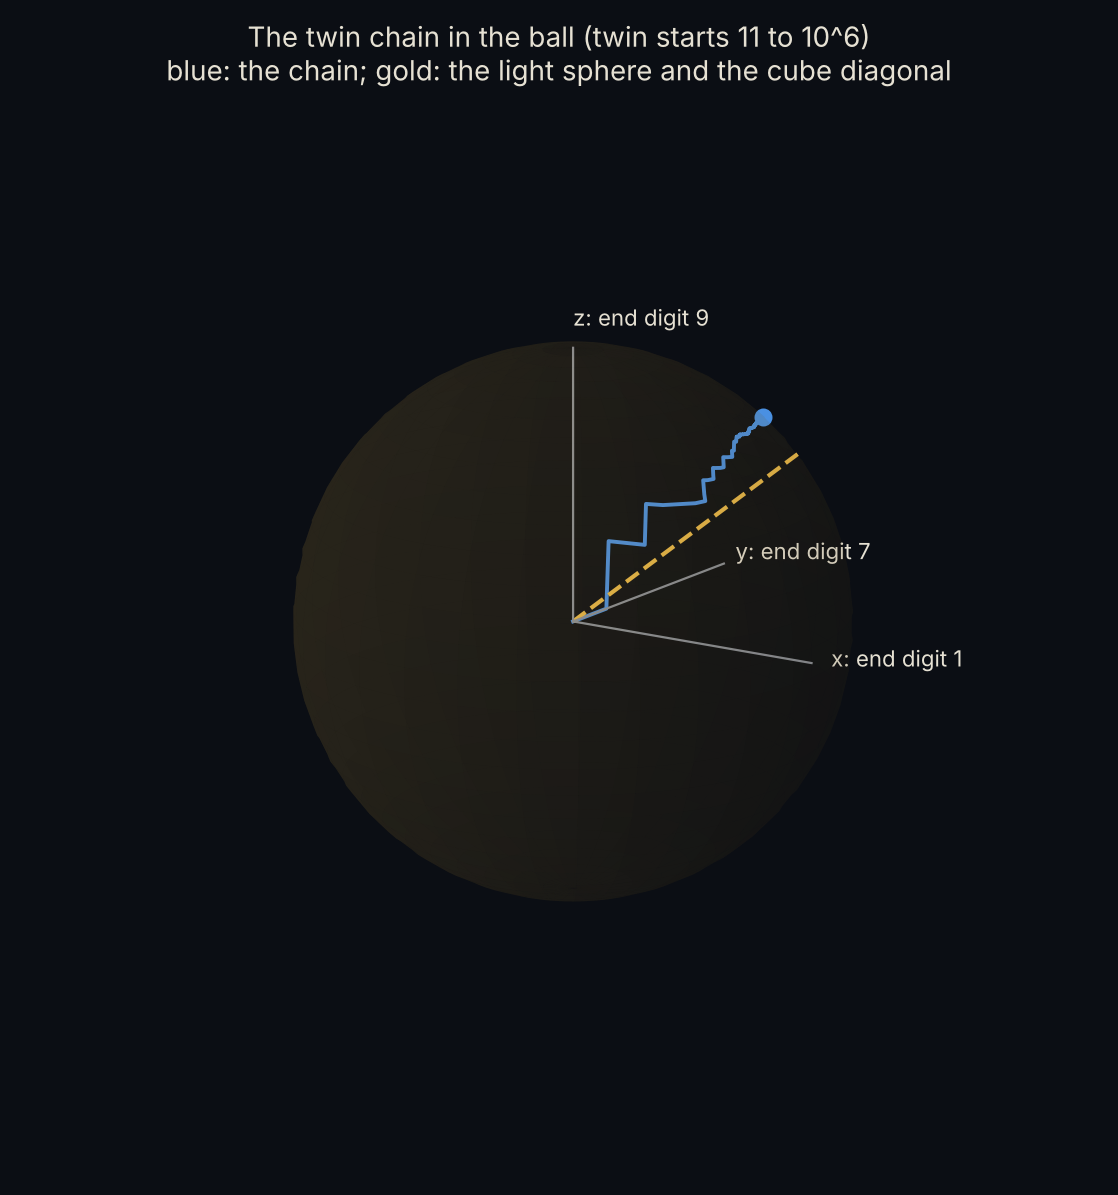
\includegraphics[width=0.62\textwidth]{fig/f1_chain_ball.png}
\caption{The twin chain to $10^6$ in the Poincar\'e ball. Blue: the walker; gold: the light sphere and the cube diagonal.}\label{fig:ball}\end{figure}

\begin{figure}[h!]\centering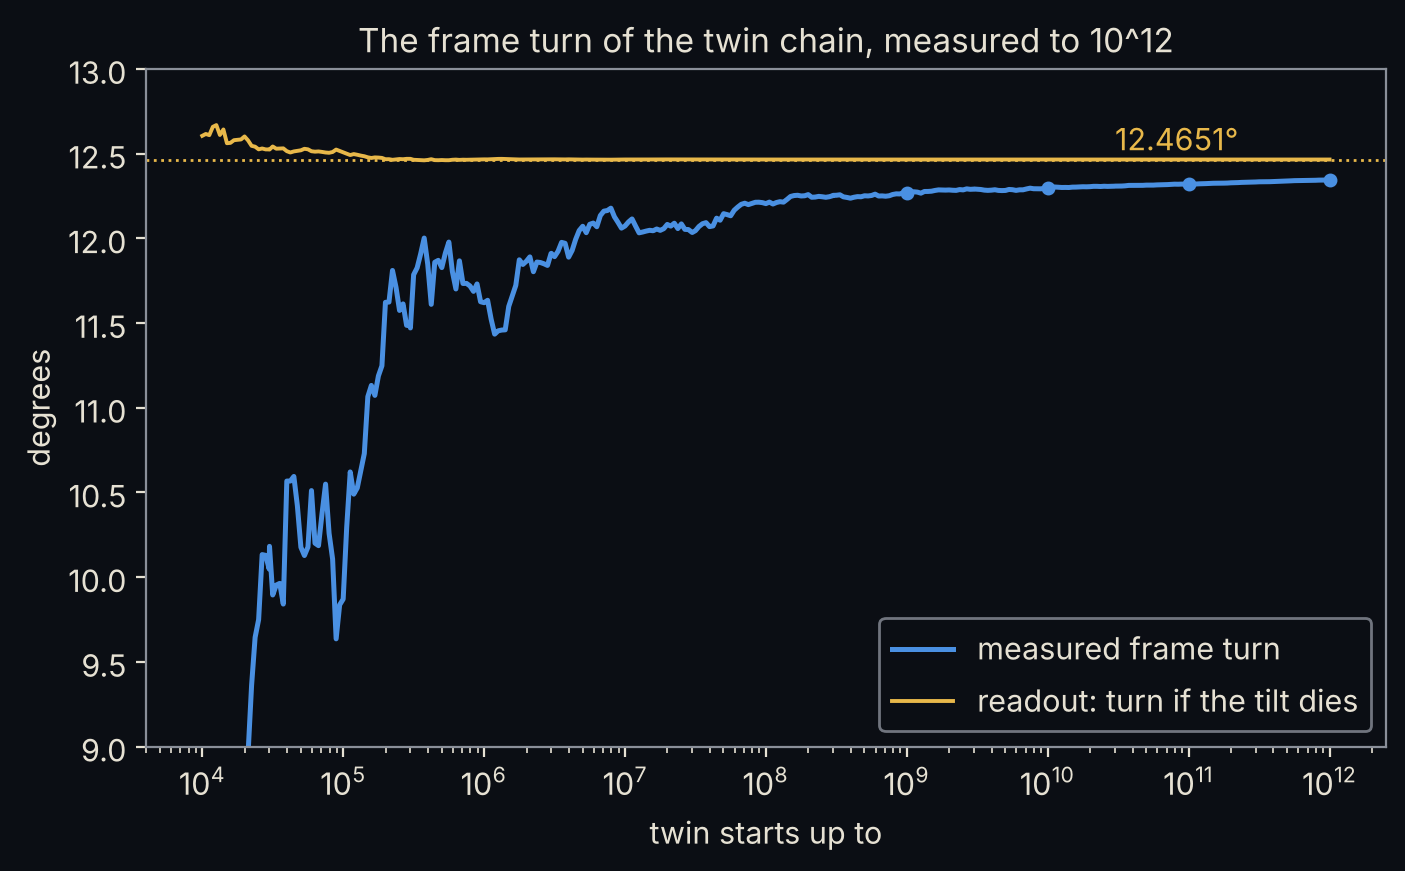
\includegraphics[width=0.9\textwidth]{fig/f2_turn_1e12.png}
\caption{The frame turn to $10^{12}$ (blue) and the readout of the turn once the tilt dies (gold).}\label{fig:turn}\end{figure}

\begin{figure}[h!]\centering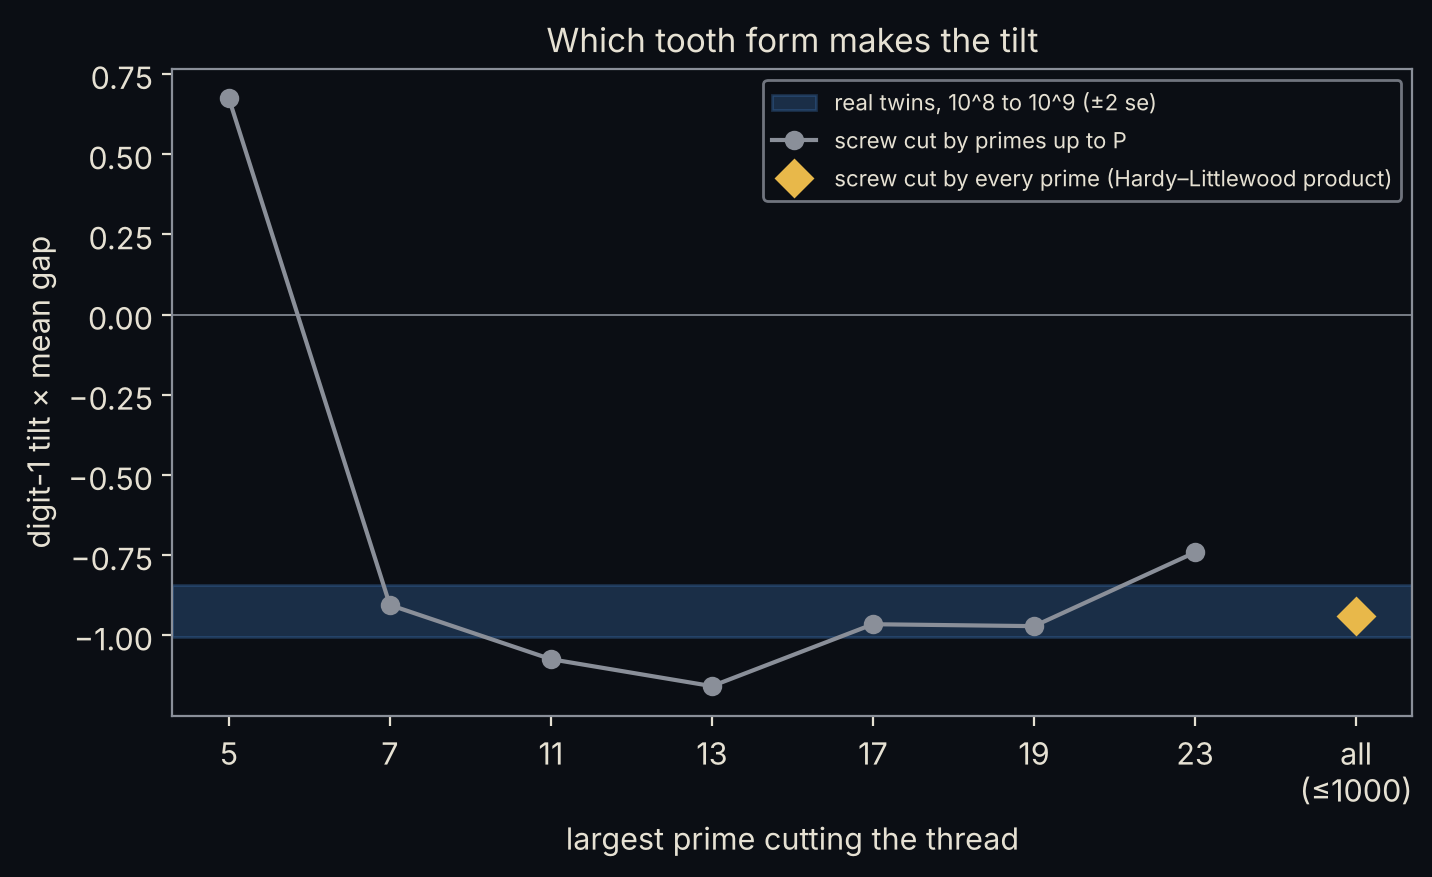
\includegraphics[width=0.85\textwidth]{fig/f3_thread_cut.png}
\caption{The thread cut prime by prime swings; cut by every prime, it lands on the twins.}\label{fig:cut}\end{figure}

\begin{figure}[h!]\centering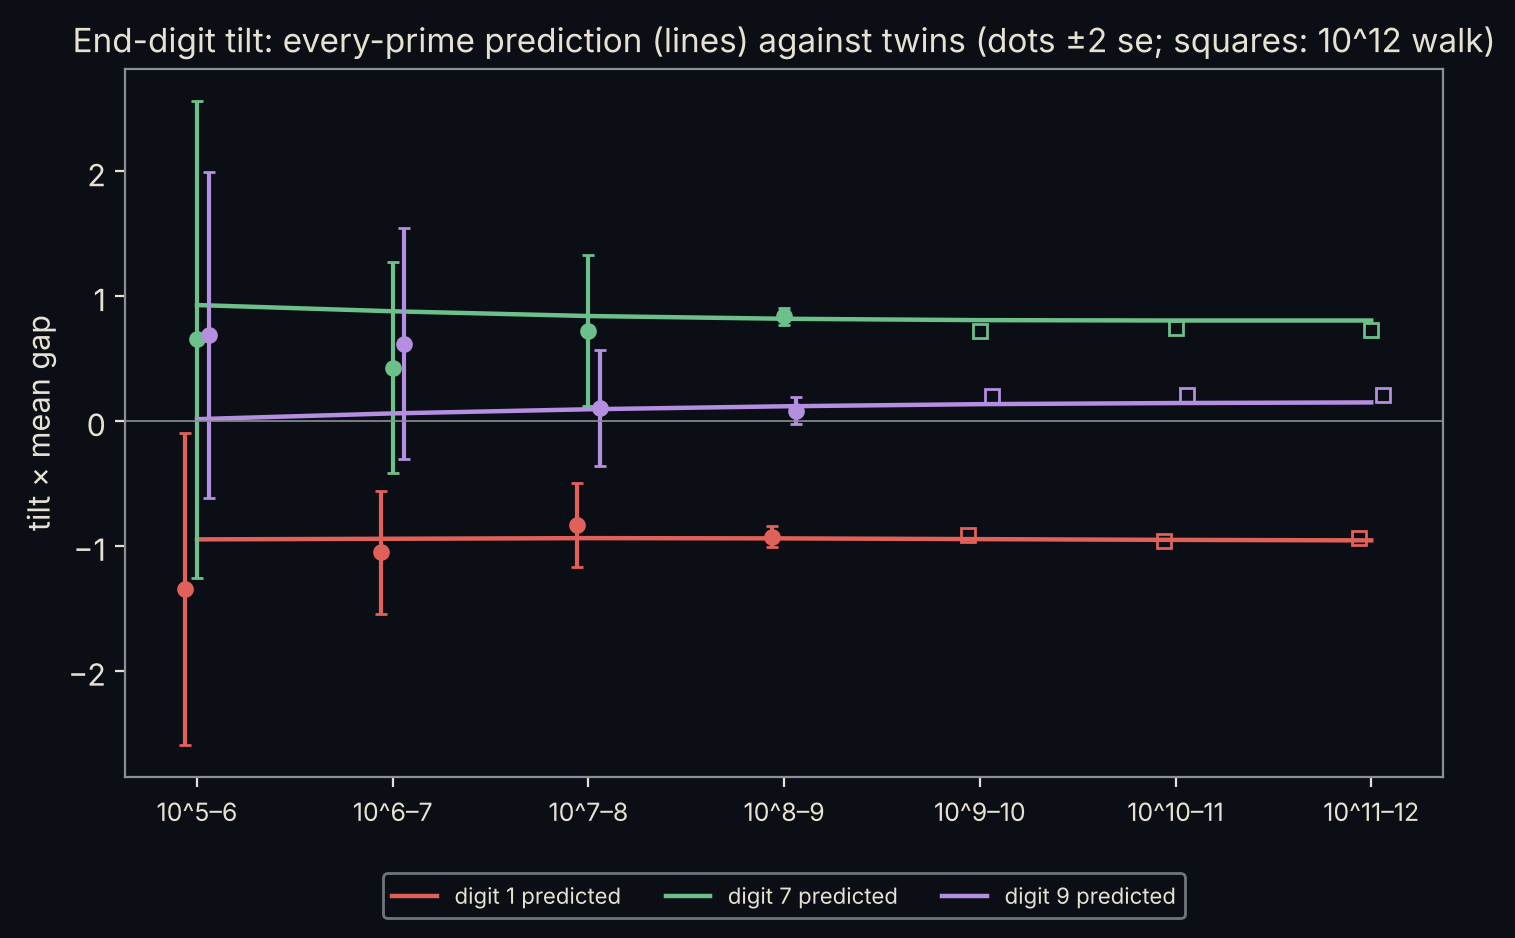
\includegraphics[width=0.95\textwidth]{fig/f4_tilt_pred_real.png}
\caption{The end-digit tilt. Lines: every-prime prediction. Dots: twin primes, with $\pm2$ se. Squares: the $10^{12}$ walk.}\label{fig:tilt}\end{figure}

\begin{figure}[h!]\centering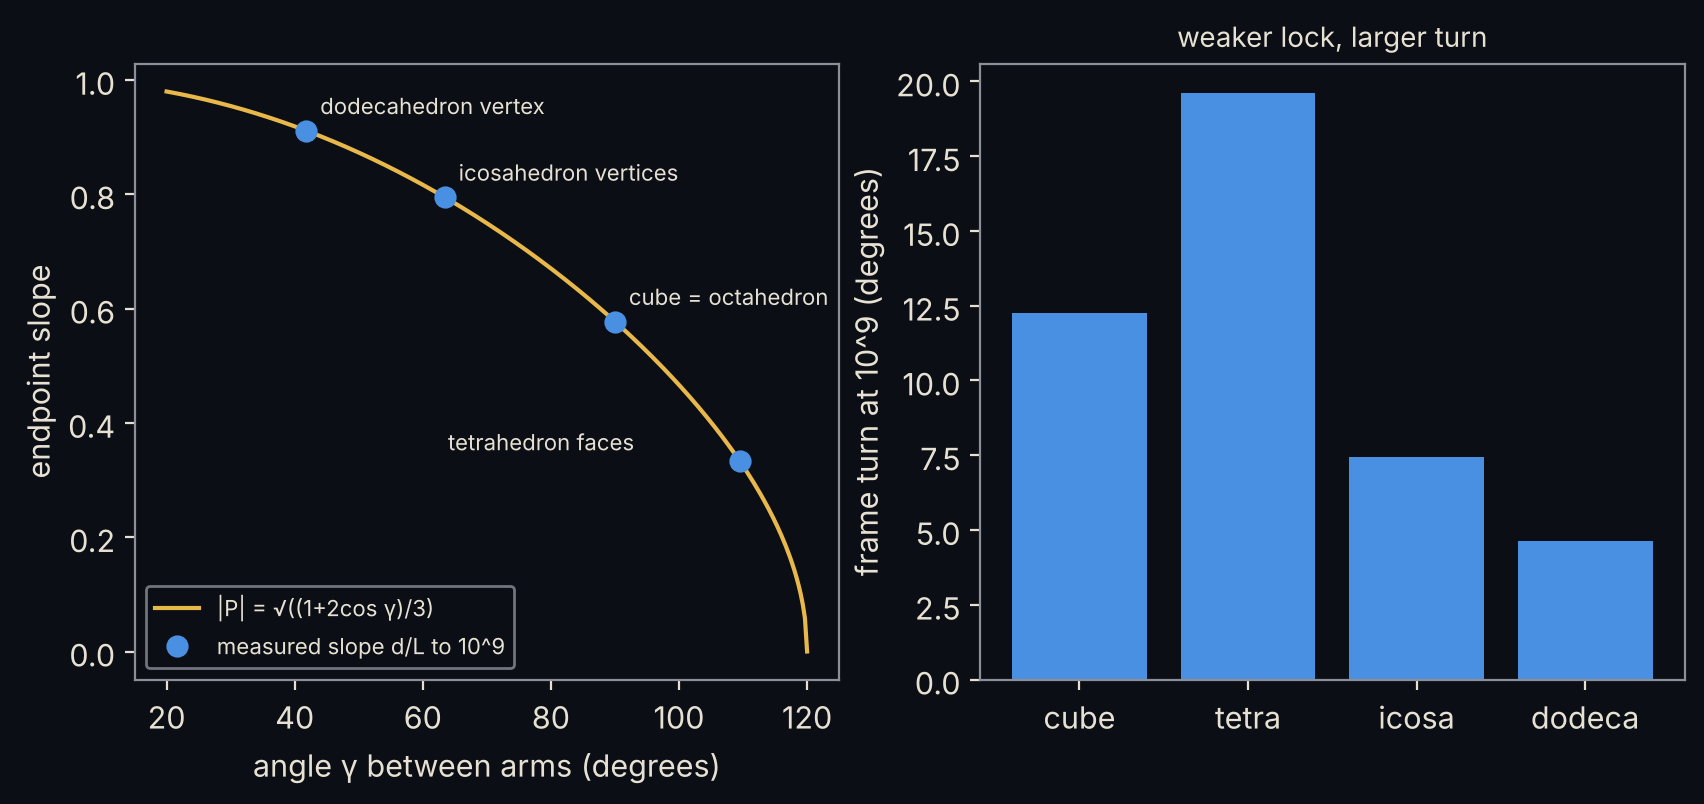
\includegraphics[width=0.95\textwidth]{fig/f5_platonic.png}
\caption{The endpoint slope against the angle between arms, for the Platonic arm sets, and the frame turn of each.}\label{fig:platonic}\end{figure}

\begin{figure}[h!]\centering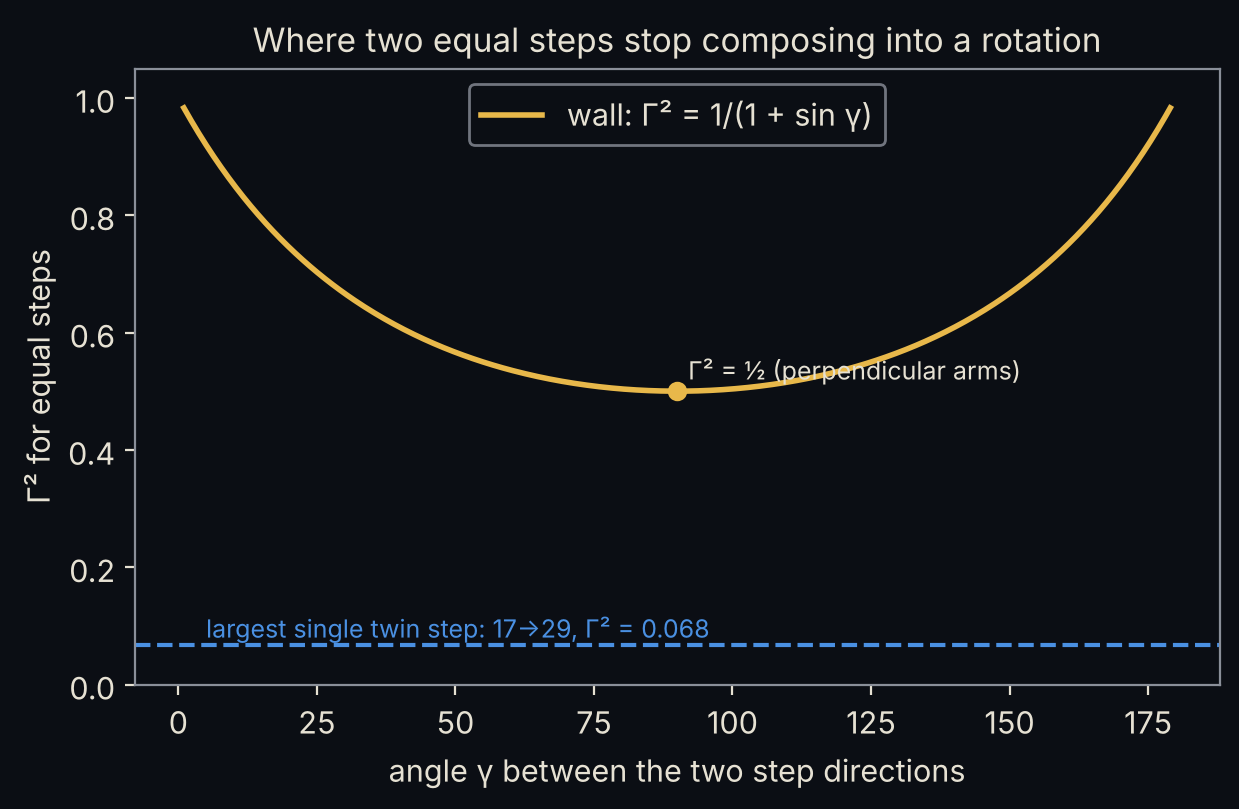
\includegraphics[width=0.8\textwidth]{fig/f6_wall.png}
\caption{The wall at any arm angle, $\Gamma^2=1/(1+\sin\gamma)$, with the largest twin step marked.}\label{fig:wall}\end{figure}

\begin{figure}[h!]\centering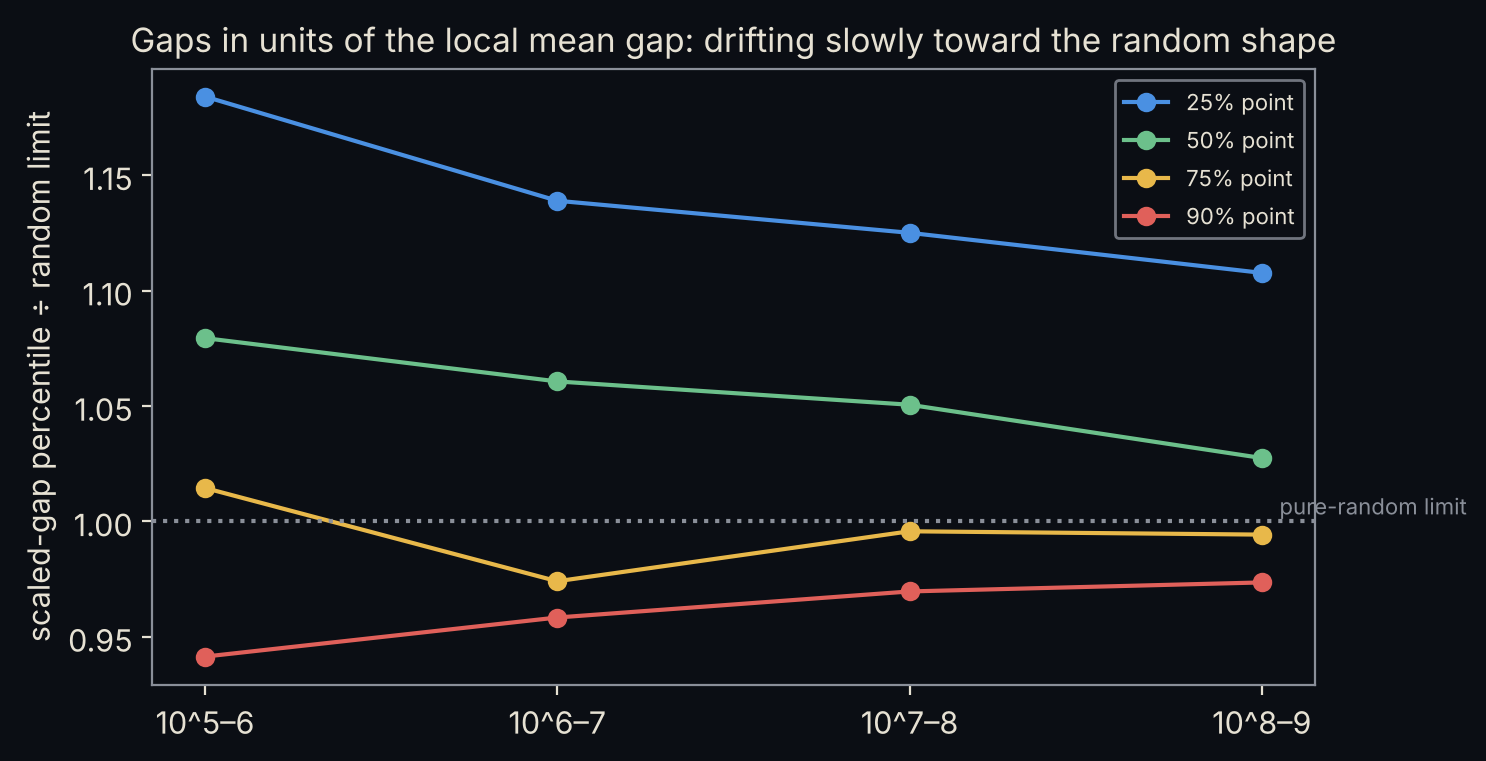
\includegraphics[width=0.8\textwidth]{fig/f7_scaled_gaps.png}
\caption{Twin gaps measured in the local mean gap, drifting slowly toward the random shape.}\label{fig:gaps}\end{figure}

\begin{figure}[h!]\centering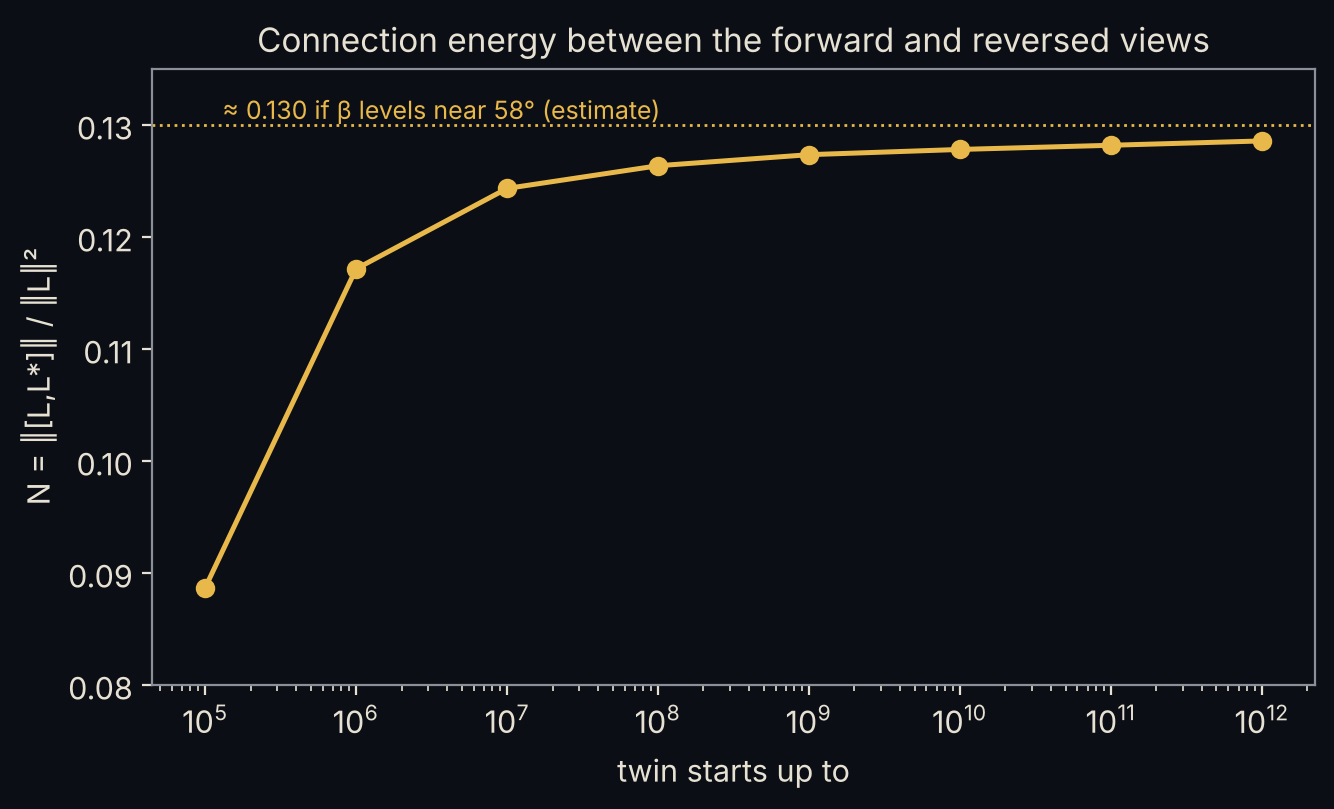
\includegraphics[width=0.8\textwidth]{fig/f8_connection_energy.png}
\caption{Connection energy between the forward and reversed readings of the chain.}\label{fig:ce}\end{figure}

\begin{figure}[h!]\centering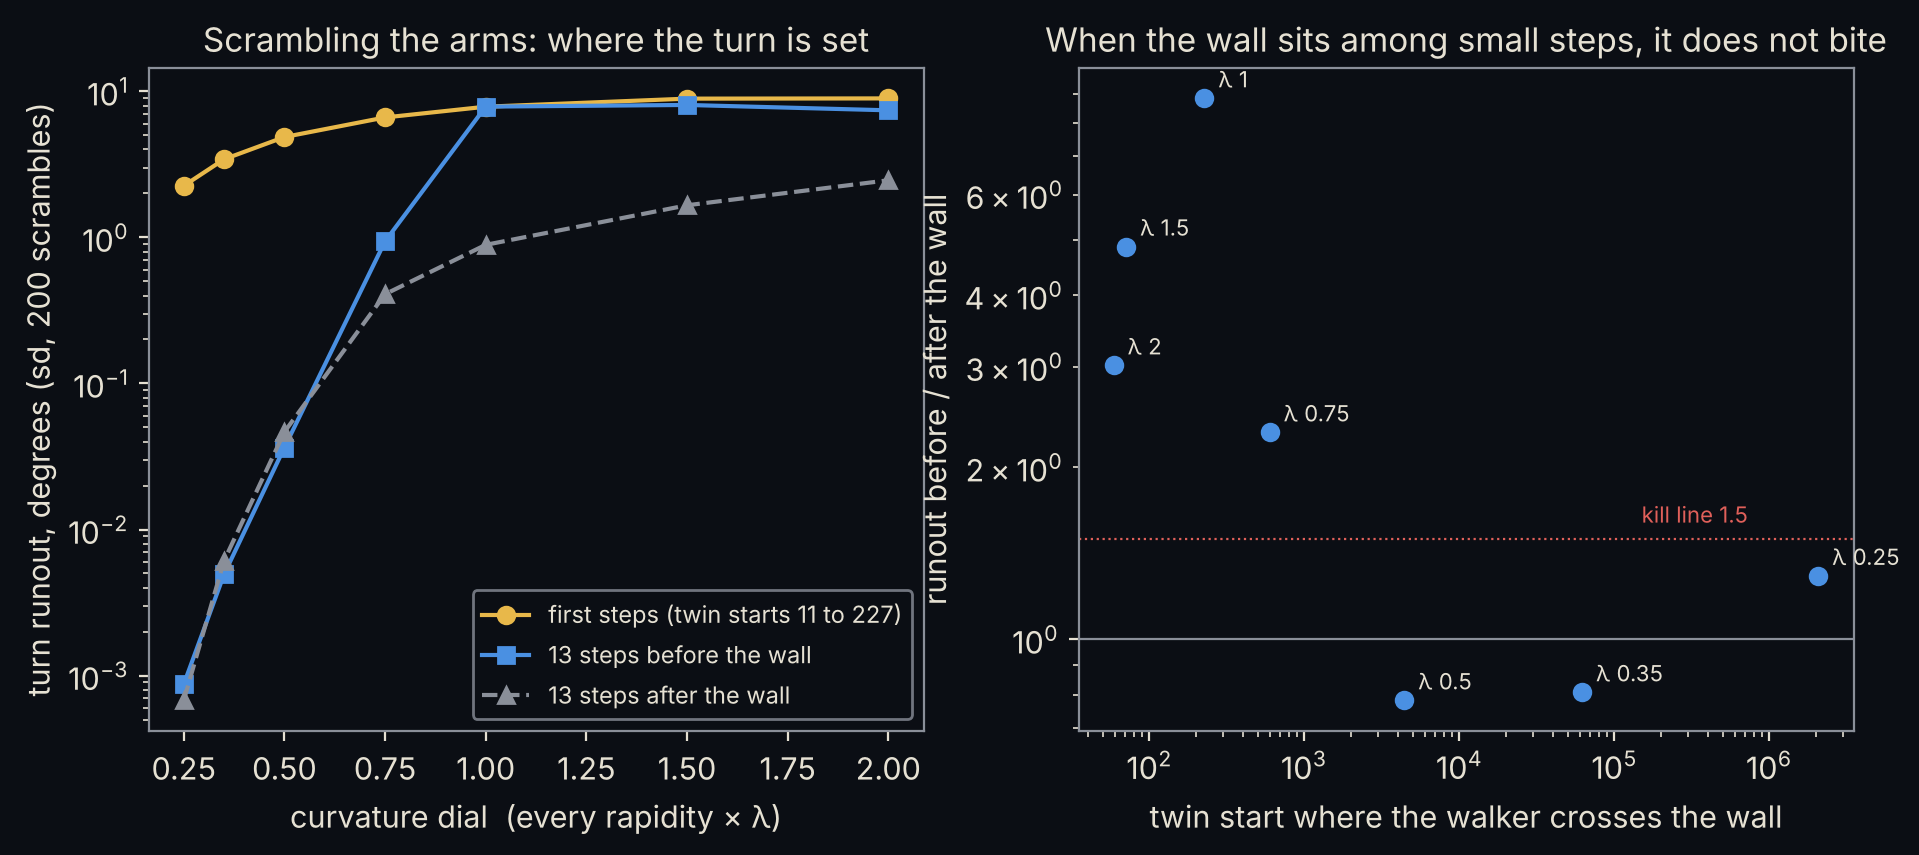
\includegraphics[width=0.98\textwidth]{fig/f9_first_cut.png}
\caption{The first cut. Left: turn runout from arm scrambles against the curvature dial. Right: before/after-wall ratio against where the wall sits.}\label{fig:firstcut}\end{figure}

\begin{figure}[h!]\centering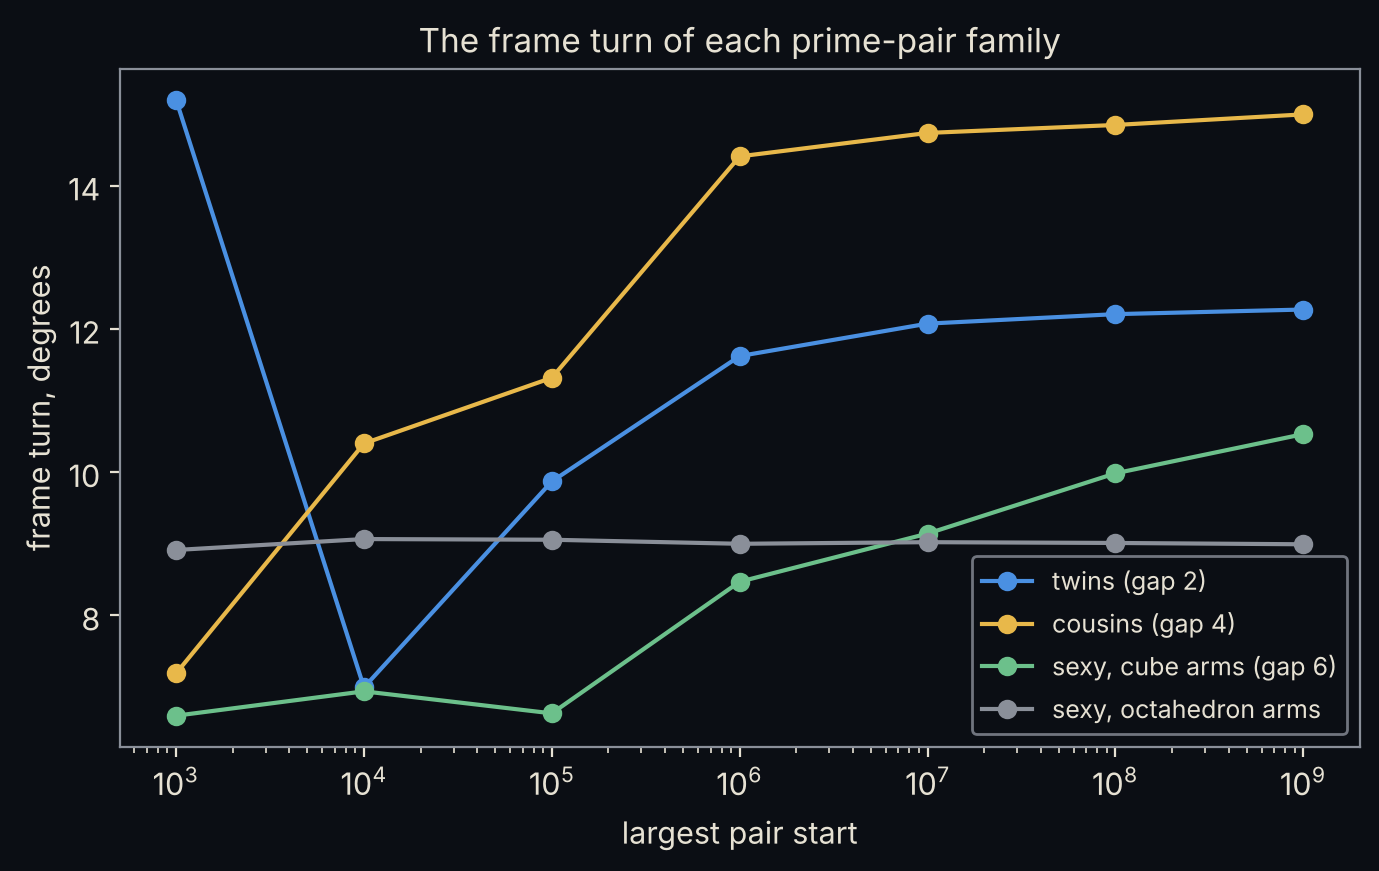
\includegraphics[width=0.8\textwidth]{fig/f10_families.png}
\caption{The frame turn of each prime-pair family, by decade.}\label{fig:families}\end{figure}

\clearpage
%=====================================================
\appendix
\section{Test register}
Every test run in this work, with the condition written before it ran, and the outcome. Where a test changed the picture, the picture above already carries the change.

\small
\begin{longtable}{p{4.2cm}p{6.2cm}p{4.3cm}}
\toprule
test & condition set before the run & outcome\\
\midrule\endhead
exact Wigner step (160 digits) & errors below $10^{-100}$ & pass ($\le2\times10^{-111}$)\\
wall at any angle & trace formula within $10^{-12}$ & pass ($1.4\times10^{-14}$)\\
frame-free form & zero error & pass\\
octant & minimum component $\ge0$ to $10^9$ & pass\\
endpoint law, all variants & $d/L$ within $1\%$ of $|P|+c/L$ & pass for mixed arms; fails for blocks and fixed steps\\
counts fix the endpoint & equal-count chain keeps $d/L$ & fails: $0.656$ vs $0.583$\\
lock on exact diagonal & heading on $(1,1,1)$ & fails: on the tilted local mean\\
mod-30 lattice tilt & sign matches & fails: wrong sign\\
bounded $d$ for $|P|=0$ & $d$ bounded & fails; $0.326\ln L$ law passes\\
$c$ from random arms & within $0.01$ & fails ($0.245\pm0.128$)\\
$c$ from real chain to $10^4$ & within $0.01$ & pass ($0.1091$ vs $0.1086$)\\
frame axis on diagonal & within $5^\circ$ & fails ($57.8^\circ$)\\
H2 tail & tail beyond $10^8$ below $10^{-4}$ & pass ($4.8\times10^{-6}$)\\
frame moves less per decade & monotone shrink & pass to $10^9$\\
walker reproduces earlier runs & to the last printed digit & pass\\
twin counts to $10^{12}$ & match published $\pi_2$ & pass\\
tilt decay $|\beta|$ & last decade $<0.5\times$ the $10^6$--$10^7$ value & pass ($0.47$)\\
curve-fit limit & spread $<0.05^\circ$ & fails (spread $0.2^\circ$): no fitted limit claimed\\
readout stability & scatter $<10^{-4}$ from $10^8$ & pass ($2.3\times10^{-5}$)\\
$c$ stability & move $<2\times10^{-4}$ from $10^9$ to $10^{12}$ & pass ($5\times10^{-5}$)\\
thread cut, random runs & one cut matches all three digits & fails\\
exact screw, $P\le19$ & digits 1, 7 within 2 se in every decade & pass\\
exact screw, $P\le23$ & stays within 2 se & fails: no finite cut is the answer\\
full product, validation & within $0.06$ of the exact 19-prime screw & pass ($0.039$)\\
full product, every decade & digits 1, 7 within 2 se, $10^5$--$10^9$ & pass\\
full product beyond $10^9$ & within $0.10$ of the walk & pass; $7/9$ split offset $\sim0.07$\\
scaled gaps & quartiles within $5\%$ across decades & fails ($6.5\%$ at 25\%): slow drift\\
connection-energy identity & matrix $=$ formula & pass ($3.5\times10^{-13}$)\\
H-CE & change shrinks $10^7\to10^9$ & pass\\
H-CE extended & change at $10^{12}<$ at $10^{10}$ & pass\\
$\beta=\arccos(1/\sqrt3)$ & within $0.5^\circ$ & fails ($57.7^\circ$)\\
\multicolumn{3}{l}{\emph{version 2}}\\
wall bite (scramble) & far runout $\ge\tfrac12$ first & pass (ratio $0.0004$)\\
curvature dial & before/after $<1.5$ wherever wall $>10^4$ & fires: wall is not the bite\\
opposite setup (late start) & before/after $<1.5$ at both starts & fires again ($0.52$, $1.30$)\\
families: slope & cousins, sexy-3 within $0.005$ of $1/\sqrt3$ & pass ($9\times10^{-5}$, $2.2\times10^{-3}$)\\
families: bounded $d$, octahedron & grows $<0.3$ & pass ($0.034$)\\
families: turn not HL & twins vs cousins differ $\ge0.3^\circ$ & pass ($2.72^\circ$)\\
families: wall crossing & $L^*\in[2.3,3.8]$ & pass for cube arms; octahedron never crosses\\
families: ordinary draw & $|z|\le3$ vs random arms & pass ($|z|\le1.49$)\\
honeycomb pentagon loop & closes, rotation $90^\circ$ & pass\\
honeycomb drift & within $2$ sd of shuffles & fires: signal at $z=-51$\\
honeycomb vs pair Markov & within $2$ sd & fires: $z=-8.7$ ($84\%$ is pair bias)\\
honeycomb vs block Markov & within $2$ sd & fires: $z=-9.05$, memory beyond pairs\\

$7/9$ split (v1 Prediction 6) & direct count closer to walk & pass\\
cousin tilt (v1 Prediction 7) & within $2$ se & pass ($|z|\le1.2$)\\
186: $\mathrm{Kl}_3$ & $\le3$, $p\le160$ & pass ($2.665$)\\
186: correlation & $\le8p\sqrt p$, $p\le160$ & pass ($4.06$)\\
186: cap rebuild, $k=40$ & lands on their values & pass\\
186: $k=39$ best trial & quotient $\ge1$ & fails ($0.99439$)\\
186: recentering & any setting reaches $0.99871$ & fires: their setup is already centred\\
\bottomrule
\end{longtable}
\normalsize

\section{Scripts and reproduction}
\sloppy
All scripts carry a \texttt{\# SCRIPT:} name and are on the branch \texttt{claude/moving-matrix-of-balls} of \texttt{dicipler-pixel/votkp-lean}, under \texttt{research/one-tree-every-shape/twin-primes-in-the-tree/}.
\begin{itemize}
\item \texttt{conv\_probe.py}, \texttt{conv\_checks.py}: first convergence argument.
\item \texttt{swarm/proof/}: exact step (160 digits), chain tests, tracking.
\item \texttt{swarm/opposite/}: other chains, random and adversarial arms.
\item \texttt{swarm/shapes/}: diagonal, Platonic arms, wall, flat readers, three-fold reading.
\item \texttt{swarm/precision/}: the $C$ walker \texttt{twinwalk.c}, the $10^{12}$ walk and its analysis.
\item \texttt{swarm/priorart/}: the connection-energy identity check.
\item \texttt{swarm/thread/}: \texttt{thread\_form.py}, \texttt{thread\_noise.py}, \texttt{thread\_exact.py}, \texttt{thread\_exact23.py}, \texttt{thread\_all.py}, \texttt{thread\_all\_decades.py}, \texttt{thread\_check\_1e12.py}, \texttt{scale\_ruler.py}, \texttt{hce\_1e12.py}.
\item \texttt{swarm/thread/} (version 2): \texttt{wall\_bite.py}, \texttt{curvature\_dial.py}, \texttt{curvature\_dial\_b.py}, \texttt{honeycomb\_534.py}, \texttt{honeycomb\_534\_markov.py}, \texttt{split\_and\_cousin.py}, with the conditions written before each run in \texttt{*\_PREREG.md}.
\item \texttt{swarm/families/}: \texttt{f1\_sieve.py}, \texttt{f2\_families.py}, \texttt{f3\_transitions.py}, \texttt{PREDICTION.txt}.
\item \texttt{gaps186/}: axiom checks, cap Gram rebuild, exact convolution, best trial, recentering scan.
\item \texttt{history/PRIMES\_HISTORY\_NOTES.md}: the history notes behind Appendix~C.
\item \texttt{paper/make\_figs.py}, \texttt{paper/make\_figs\_v2.py}: every figure.
\end{itemize}

\section{How the primes were found: a short record}
These are background notes, kept to dated records; disputed readings are marked. The full notes, with sources, are in \texttt{history/PRIMES\_HISTORY\_NOTES.md}.
\begin{itemize}
\item Old Babylonian reciprocal tables (about 1800 BCE) list only numbers built from $2,3,5$; $7$ is marked as having no reciprocal. The first written prime arithmetic is the wheel $2\cdot3\cdot5=30$, the same wheel the twin classes $11,17,29\pmod{30}$ come from, with $7$ the first number left out. In Section~\ref{sec:thread}, cutting the thread by $7$ is what gives the tilt its real sign.
\item Ishango bone (about 20{,}000 years ago): one column reads $11,13,17,19$. Whether that is deliberate is disputed.
\item Euclid, \emph{Elements} VII.31--32, IX.20, IX.36 (about 300 BCE); Eratosthenes' sieve (about 240 BCE).
\item Sunzi (3rd--5th century) and Qin Jiushao (1247): the remainder theorem, which is how the mod-30 wheel is assembled.
\item Aryabhata (499) and Brahmagupta (628): linear congruences.
\item Euler (1737): the product over all primes, the shape of the every-prime cut of Section~\ref{sec:thread}.
\item Polignac (1849): every even gap occurs infinitely often.
\item Brun (1919): the twin reciprocals converge, the same reason the chain's turn converges.
\item Hardy and Littlewood (1923): the local factors used for the tilt.
\item Zhang (2013); Maynard, Tao and Polymath (2014): bounded gaps, $246$.
\item Lemke Oliver and Soundararajan (2016): consecutive-prime end-digit bias.
\item Stadlmann (2026): $240$; Axiom Math: $212$ (claimed); OpenAI: $186$ (conditional on three stated assumptions; Section~\ref{sec:186}). Gap $2$ is still open.
\end{itemize}

\begin{thebibliography}{99}\small
\bibitem{HL} G.~H.~Hardy and J.~E.~Littlewood, Some problems of `partitio numerorum' III, \emph{Acta Math.} 44 (1923) 1--70.
\bibitem{Brun} V.~Brun, La s\'erie $1/5+1/7+\dots$ o\`u les d\'enominateurs sont nombres premiers jumeaux est convergente, \emph{Bull. Sci. Math.} 43 (1919).
\bibitem{RM} H.~Robbins and S.~Monro, A stochastic approximation method, \emph{Ann. Math. Statist.} 22 (1951).
\bibitem{KC} H.~J.~Kushner and D.~S.~Clark, \emph{Stochastic Approximation Methods for Constrained and Unconstrained Systems}, Springer, 1978.
\bibitem{B96} M.~Bena\"im, A dynamical system approach to stochastic approximations, \emph{SIAM J. Control Optim.} 34 (1996).
\bibitem{B99} M.~Bena\"im, Dynamics of stochastic approximation algorithms, \emph{S\'em. Probab.} XXXIII, LNM 1709 (1999).
\bibitem{LOS} R.~J.~Lemke Oliver and K.~Soundararajan, Unexpected biases in the distribution of consecutive primes, \emph{PNAS} 113 (2016); arXiv:1603.03720.
\bibitem{Sahoo} Sahoo, twin primes in residue classes, arXiv:2111.09053.
\bibitem{Fraile} Fraile et al., prime walks by last digit, arXiv:2105.12547; arXiv:2506.15357.
\bibitem{Holt} Holt, gap populations and prime biases, arXiv:2405.03540.
\bibitem{PP} V.~Palge and C.~Pfeifer, Thomas--Wigner rotation as holonomy, arXiv:2310.08121.
\bibitem{MRT} K.~Matom\"aki, M.~Radziwi\l\l\ and T.~Tao, correlations of the von Mangoldt and higher divisor functions, arXiv:1707.01315.
\bibitem{Lu} Lu, Counts converge, spacings do not, ICML 2026 poster.
\bibitem{BFT} W.~Banks, T.~Freiberg and C.~Turnage-Butterbaugh, Consecutive primes in tuples, \emph{Acta Arith.} 167 (2015).
\bibitem{Gran} A.~Granville, Harald Cram\'er and the distribution of prime numbers, \emph{Scand. Actuar. J.} (1995).
\bibitem{Ungar} A.~A.~Ungar, \emph{Analytic Hyperbolic Geometry and Albert Einstein's Special Theory of Relativity}, World Scientific, 2008.
\bibitem{JB1} J.~Beasley, Non-normality is connection energy, Zenodo, 10.5281/zenodo.22803572.
\bibitem{JB2} J.~Beasley, VOTKP; Two Trees in One Ball; Matter at a Scale; Dirac Time (Zenodo and GitHub, \texttt{dicipler-pixel}).
\bibitem{OAI} OpenAI, Improved short gaps between primes, and Lean certificate, \texttt{github.com/openai/PrimeGaps186} (2026).
\bibitem{Stad} J.~Stadlmann, Bounded gaps between primes, arXiv:2608.31126.
\bibitem{May} J.~Maynard, Small gaps between primes, \emph{Ann. of Math.} 181 (2015).
\bibitem{Poly} D.~H.~J.~Polymath, Variants of the Selberg sieve, and bounded intervals containing many primes, \emph{Res. Math. Sci.} 1 (2014).
\bibitem{FKM} \'E.~Fouvry, E.~Kowalski and Ph.~Michel, Algebraic trace functions over the primes, arXiv:1207.0617.
\bibitem{Cox} H.~S.~M.~Coxeter, \emph{Regular Honeycombs in Hyperbolic Space}, Proc. ICM Amsterdam (1954); \emph{Regular Polytopes}, Dover, 1973.
\bibitem{Sutherland} A.~V.~Sutherland, narrow admissible tuples, OEIS A008407.
\end{thebibliography}
\end{document}
